\documentclass[12pt,a4paper]{article}

\usepackage{etoolbox}
\providetoggle{long}
%\settoggle{long}{true}
\settoggle{long}{false}

\newcommand{\komentar}[1]{\textcolor{red}{[#1]}} %for displaying red texts

\usepackage{fullpage}
\usepackage{fancyhdr}
\usepackage{enumerate}
\pagestyle{fancy}
%\fancyfoot[ROF,REF]{\tiny Pripravil Martin Milani\v c.}

\usepackage[slovene]{babel} % slovenske nastavitve (naslovi, deljenje besed ...)
\usepackage[utf8]{inputenc}
\usepackage{amsfonts,amssymb}
\usepackage{graphicx}
\usepackage{amsmath,amssymb,amsthm}
\usepackage{epsf}
\usepackage{epsfig}
\usepackage{graphics}
\usepackage{color}
\usepackage{comment}
%\usepackage{times}
%\usepackage{txfonts}
\def\P {{\cal P}}
\def\ali {{~\vee~}}
\def\inn {{~\wedge~}}
\def\sledi {{~\Rightarrow~}}
\def\brez {{\,\setminus\,}}
\def\cee {{~\Leftrightarrow~}}
\def\zgled{\noindent{\bf\color{blue} Zgled: }}
\def\kz{{\hfill{\color{blue}$\blacktriangle$}}}% konec zgleda
%\parskip=7pt
%
%\textwidth=17cm\textheight=22cm\parindent=15pt\parskip=5pt
%\oddsidemargin=-5mm  \headheight=0pt \pagestyle{plain}
\newtheorem*{trditev}{Trditev}
\newtheorem*{izrek}{Izrek}
\newtheorem*{problem}{Naloga}
\newtheorem*{lema}{Lema}
\newtheorem*{posledica}{Posledica}
\newtheorem*{definicija}{Definicija}

\def\proofname{Dokaz}

\begin{document}

\section{Matematična logika}

\iftoggle{long}{\komentar{Skrajšano: OD TU}\\}

\iftoggle{long}{
{\color{blue}
Kaj je izjava? {\em Trdilna izjava}, ki je bodisi pravilna ali pa nepravilna.\footnote{Izjave boste podrobneje obravnavali na uvodnem predavanju pri Analizi I.}

\medskip
Prispevek logike k znanju je v odkrivanju novih izjav, ki so logične posledice drugih.
\begin{itemize}
  \item Celotno teorijo naravnih števil je moč zgraditi iz 5 osnovnih izjav,
  ki jih običajno imenujemo Peanovi aksiomi. Teh pet izjav lahko z besedico ``in"~povežemo v eno samo
  izjavo.
  \item Hilbert je pokazal, da je vso kopico izrekov elementarne geometrije moč dokazati iz 20 aksiomov
  (osnovnih izjav).
  \item V splošnem so matematične strukture definirane s peščico aksiomov,
  iz katerih se s pomočjo logičnega sklepanja izpelje izreke in gradi teorije.
\end{itemize}

O razvoju logike in teorije množic si lahko preberete v Prijateljevi knjigi (Osnove matematične logike, 1.~poglavje, 2.~podpoglavje).

\subsection{Osnovne povezave in pravilnostne tabele}

{\bf \underline{Negacija:}} Ne $A$; ni res, da $A$

Oznaka: $\neg A$.

$\neg A$ je negacija izjave $A$. Izjava $\neg A$ je pravilna, če je $A$ nepravilna, in je nepravilna,
če je $A$ pravilna.

Zgled: {\em Jutri bo dež. Negacija: Jutri ne bo dežja. (Ni res, da bo jutri dež.)}

\medskip
Vrednost vsake sestavljene izjave je enolično določena z vrednostmi osnovnih izjav, ki v njej nastopajo.
Za nazoren pregled te odvisnosti si pomagamo s t.i.~{\em pravilnostnimi tabelami}.
Dogovorimo se, da bomo vrednost {\em pravilno} označevali z~1, vrednost {\em nepravilno} pa z~0.

Pravilnostna tabela za negacijo:
$$\begin{tabular}{c|c|c}
  \hline
  % after \\: \hline or \cline{col1-col2} \cline{col3-col4} ...
   & $A$ & $\neg A$ \\
  \hline
  1. & 1 & 0 \\
  2. & 0 & 1 \\
\end{tabular}$$

\medskip
{\bf \underline{Konjunkcija:}} $A$ in $B$

Oznaka: $A\inn  B$

$A\wedge B$ je konjunkcija izjav $A$ in $B$. Ta sestavljena izjava je pravilna,
kadar sta obe izjavi $A$ in $B$ pravilni, in nepravilna sicer.

Zgled: {\em Sneg pada. Veter piha. Konjunkcija: Sneg pada in veter piha.}

\medskip
{\bf \underline{Disjunkcija:}} $A$ ali $B$ (inkluzivno)

Oznaka: $A\ali B$

$A\ali B$ je disjunkcija izjav $A$ in $B$. Ta sestavljena izjava je pravilna,
brž ko je ena izmed izjav  $A$ in $B$ pravilna, in nepravilna sicer.

Zgled: {\em Janez bo jutri vprašan fiziko. Janez bo jutri vprašan matematiko.
Disjunkcija: Janez bo jutri vprašan fiziko ali matematiko.}

\medskip
{\bf \underline{Implikacija:}} Če $A$, potem $B$

Oznaka: $A\sledi B$

$A\sledi B$ je implikacija izjav $A$ in $B$. Ta sestavljena izjava je nepravilna,
kadar je $A$ pravilna, $B$ pa nepravilna. V vseh ostalih primerih je pravilna.

$A$ - antecedens, zadostni pogoj

$B$ - konsekvens

\zgled: {\em Če Andrej naredi maturo, potem mu kupim kolo.}

\medskip
{\bf \underline{Ekvivalenca:}} $A$ če in samo če $B$

Oznaka: $A\cee B$

$A\cee B$ je ekvivalenca izjav $A$ in $B$. Ta sestavljena izjava je pravilna,
kadar sta izjavi $A$ in $B$ ali obe pravilni ali obe nepravilni.
V vseh ostalih primerih je nepravilna.

"$A\cee B$" beremo:

$A$ če in samo če $B$

$A$ tedaj in samo tedaj kot $B$

$A$ natanko tedaj kot $B$

\zgled {\em Andreju kupim kolo, če in samo če naredi maturo.}

\medskip
{\bf Pravilnostne tabele za konjuncijo, disjunkcijo, implikacijo in ekvivalenco:}
$$\begin{tabular}{c|c|c|c|c|c}
  \hline
  % after \\: \hline or \cline{col1-col2} \cline{col3-col4} ...
   & $A, B$ & $A \inn B$ & $A \ali B$ & $A \sledi B$ & $A \cee B$ \\
  \hline
  1. & 1, 1 & 1 & 1 & 1 & 1 \\
  2. & 1, 0 & 0 & 1 & 0 & 0  \\
  3. & 0, 1 & 0 & 1 & 1 & 0  \\
  4. & 0, 0 & 0 & 0 & 1 & 1 \\
\end{tabular}$$

\medskip

Izjave, dobljene z uprabo $5$ osnovnih povezav, so {\it sestavljene}. V splošnem pravimo, da je dana izjava {\it sestavljena}, če je izid
zaporedne uporabe $5$ osnovnih povezav na osnovnih izjavah $A_1,\ldots, A_n$, pa tudi na izjavah, ki smo jih že prej napravili.
Dvomom o tem, katera povezava sledi prej in katera pozneje, se izognemo z uporabo oklepajev.
Uporabo oklepajev pa z uporabo naslednjega dogovora omejimo, kolikor se da:
\begin{itemize}
  \item Kadar izjava nastopa osamljeno, je ne oklenemo z oklepaji:

  npr.: namesto $(A\inn B)$ pišemo $A\inn B$

  \item Kadar ista vrsta povezave nastopi večkrat zapored, jo obravnavamo z leve proti desni.

  npr.: namesto $((A\inn B) \inn C) \inn D$ pišemo $A\inn B \inn C\inn D$

  \item Upoštevamo naslednji prednostni red operacij:
  $\neg$, $\ali$, $\inn$, $\sledi$, $\cee$ (v vsaki sestavljeni izjavi najprej upoštevamo negacije, za njimi disjunkcije itd.)

  npr.: namesto $(A\inn B) \sledi (\neg C)$ pišemo  $A\inn B \sledi\neg C$
\end{itemize}

\medskip
Pravilnostne tabele lahko zapišemo tudi za sestavljene izjave, z uporabo poljubnega
zaporedja, s katerim sestavimo izjavo.

\zgled
\begin{equation}\label{eq:izjava2}
(A \sledi B) \inn (B\sledi C) \inn  (\neg A \ali C)
\end{equation}

$$\begin{tabular}{c|c|c|c|c|c|c|c}
  \hline
  % after \\: \hline or \cline{col1-col2} \cline{col3-col4} ...
   & $A, B, C$ & $A \sledi B$ & $B \sledi C$ & $(A \sledi B) \inn (B\sledi C)$ & $\neg A$ & $\neg A \ali C$ & $(\ref{eq:izjava2})$\\
  \hline
  1. & 1, 1, 1 & 1 & 1 & 1 & 0 & 1 & 1 \\
  2. & 1, 1, 0 & 1 & 0 & 0 & 0 & 0 & 0 \\
  3. & 1, 0, 1 & 0 & 1 & 0 & 0 & 1 & 0 \\
  4. & 1, 0, 0 & 0 & 1 & 0 & 0 & 0 & 0 \\
  5. & 0, 1, 1 & 1 & 1 & 1 & 1  & 1 & 1 \\
  6. & 0, 1, 0 & 1 & 0 & 0 & 1  & 1 & 0 \\
  7. & 0, 0, 1 & 1 & 1 & 1 & 1  & 1 & 1 \\
  8. & 0, 0, 0 & 1 & 1 & 1 & 1  & 1 & 1 \\
\end{tabular}$$
}}
{
Kaj je izjava? {\em Trdilna izjava}, ki je bodisi pravilna ali pa nepravilna.\footnote{Izjave boste podrobneje obravnavali na uvodnem predavanju pri Analizi I.}

\medskip
Prispevek logike k znanju je v odkrivanju novih izjav, ki so logične posledice drugih.
\begin{itemize}
  \item Celotno teorijo naravnih števil je moč zgraditi iz 5 osnovnih izjav,
  ki jih običajno imenujemo Peanovi aksiomi. Teh pet izjav lahko z besedico ``in"~povežemo v eno samo
  izjavo.
  \item Hilbert je pokazal, da je vso kopico izrekov elementarne geometrije moč dokazati iz 20 aksiomov
  (osnovnih izjav).
  \item V splošnem so matematične strukture definirane s peščico aksiomov,
  iz katerih se s pomočjo logičnega sklepanja izpelje izreke in gradi teorije.
\end{itemize}

O razvoju logike in teorije množic si lahko preberete v Prijateljevi knjigi (Osnove matematične logike, 1.~poglavje, 2.~podpoglavje).

\subsection{Osnovne povezave in pravilnostne tabele}

{\bf \underline{Negacija:}} Ne $A$; ni res, da $A$

Oznaka: $\neg A$.

$\neg A$ je negacija izjave $A$. Izjava $\neg A$ je pravilna, če je $A$ nepravilna, in je nepravilna,
če je $A$ pravilna.

Zgled: {\em Jutri bo dež. Negacija: Jutri ne bo dežja. (Ni res, da bo jutri dež.)}

\medskip
Vrednost vsake sestavljene izjave je enolično določena z vrednostmi osnovnih izjav, ki v njej nastopajo.
Za nazoren pregled te odvisnosti si pomagamo s t.i.~{\em pravilnostnimi tabelami}.
Dogovorimo se, da bomo vrednost {\em pravilno} označevali z~1, vrednost {\em nepravilno} pa z~0.

Pravilnostna tabela za negacijo:
$$\begin{tabular}{c|c|c}
  \hline
  % after \\: \hline or \cline{col1-col2} \cline{col3-col4} ...
   & $A$ & $\neg A$ \\
  \hline
  1. & 1 & 0 \\
  2. & 0 & 1 \\
\end{tabular}$$

\medskip
{\bf \underline{Konjunkcija:}} $A$ in $B$

Oznaka: $A\inn  B$

$A\wedge B$ je konjunkcija izjav $A$ in $B$. Ta sestavljena izjava je pravilna,
kadar sta obe izjavi $A$ in $B$ pravilni, in nepravilna sicer.

Zgled: {\em Sneg pada. Veter piha. Konjunkcija: Sneg pada in veter piha.}

\medskip
{\bf \underline{Disjunkcija:}} $A$ ali $B$ (inkluzivno)

Oznaka: $A\ali B$

$A\ali B$ je disjunkcija izjav $A$ in $B$. Ta sestavljena izjava je pravilna,
brž ko je ena izmed izjav  $A$ in $B$ pravilna, in nepravilna sicer.

Zgled: {\em Janez bo jutri vprašan fiziko. Janez bo jutri vprašan matematiko.
Disjunkcija: Janez bo jutri vprašan fiziko ali matematiko.}

\medskip
{\bf \underline{Implikacija:}} Če $A$, potem $B$

Oznaka: $A\sledi B$

$A\sledi B$ je implikacija izjav $A$ in $B$. Ta sestavljena izjava je nepravilna,
kadar je $A$ pravilna, $B$ pa nepravilna. V vseh ostalih primerih je pravilna.

$A$ - antecedens, zadostni pogoj

$B$ - konsekvens

\zgled: {\em Če Andrej naredi maturo, potem mu kupim kolo.}

\medskip
{\bf \underline{Ekvivalenca:}} $A$ če in samo če $B$

Oznaka: $A\cee B$

$A\cee B$ je ekvivalenca izjav $A$ in $B$. Ta sestavljena izjava je pravilna,
kadar sta izjavi $A$ in $B$ ali obe pravilni ali obe nepravilni.
V vseh ostalih primerih je nepravilna.

"$A\cee B$" beremo:

$A$ če in samo če $B$

$A$ tedaj in samo tedaj kot $B$

$A$ natanko tedaj kot $B$

\zgled {\em Andreju kupim kolo, če in samo če naredi maturo.}

\medskip
{\bf Pravilnostne tabele za konjuncijo, disjunkcijo, implikacijo in ekvivalenco:}
$$\begin{tabular}{c|c|c|c|c|c}
  \hline
  % after \\: \hline or \cline{col1-col2} \cline{col3-col4} ...
   & $A, B$ & $A \inn B$ & $A \ali B$ & $A \sledi B$ & $A \cee B$ \\
  \hline
  1. & 1, 1 & 1 & 1 & 1 & 1 \\
  2. & 1, 0 & 0 & 1 & 0 & 0  \\
  3. & 0, 1 & 0 & 1 & 1 & 0  \\
  4. & 0, 0 & 0 & 0 & 1 & 1 \\
\end{tabular}$$

\medskip

Izjave, dobljene z uprabo $5$ osnovnih povezav, so {\it sestavljene}. V splošnem pravimo, da je dana izjava {\it sestavljena}, če je izid
zaporedne uporabe $5$ osnovnih povezav na osnovnih izjavah $A_1,\ldots, A_n$, pa tudi na izjavah, ki smo jih že prej napravili.
Dvomom o tem, katera povezava sledi prej in katera pozneje, se izognemo z uporabo oklepajev.
Uporabo oklepajev pa z uporabo naslednjega dogovora omejimo, kolikor se da:
\begin{itemize}
  \item Kadar izjava nastopa osamljeno, je ne oklenemo z oklepaji:

  npr.: namesto $(A\inn B)$ pišemo $A\inn B$

  \item Kadar ista vrsta povezave nastopi večkrat zapored, jo obravnavamo z leve proti desni.

  npr.: namesto $((A\inn B) \inn C) \inn D$ pišemo $A\inn B \inn C\inn D$

  \item Upoštevamo naslednji prednostni red operacij:
  $\neg$, $\ali$, $\inn$, $\sledi$, $\cee$ (v vsaki sestavljeni izjavi najprej upoštevamo negacije, za njimi disjunkcije itd.)

  npr.: namesto $(A\inn B) \sledi (\neg C)$ pišemo  $A\inn B \sledi\neg C$
\end{itemize}

\medskip
Pravilnostne tabele lahko zapišemo tudi za sestavljene izjave, z uporabo poljubnega
zaporedja, s katerim sestavimo izjavo.

\zgled
\begin{equation}\label{eq:izjava2}
(A \sledi B) \inn (B\sledi C) \inn  (\neg A \ali C)
\end{equation}

$$\begin{tabular}{c|c|c|c|c|c|c|c}
  \hline
  % after \\: \hline or \cline{col1-col2} \cline{col3-col4} ...
   & $A, B, C$ & $A \sledi B$ & $B \sledi C$ & $(A \sledi B) \inn (B\sledi C)$ & $\neg A$ & $\neg A \ali C$ & $(\ref{eq:izjava2})$\\
  \hline
  1. & 1, 1, 1 & 1 & 1 & 1 & 0 & 1 & 1 \\
  2. & 1, 1, 0 & 1 & 0 & 0 & 0 & 0 & 0 \\
  3. & 1, 0, 1 & 0 & 1 & 0 & 0 & 1 & 0 \\
  4. & 1, 0, 0 & 0 & 1 & 0 & 0 & 0 & 0 \\
  5. & 0, 1, 1 & 1 & 1 & 1 & 1  & 1 & 1 \\
  6. & 0, 1, 0 & 1 & 0 & 0 & 1  & 1 & 0 \\
  7. & 0, 0, 1 & 1 & 1 & 1 & 1  & 1 & 1 \\
  8. & 0, 0, 0 & 1 & 1 & 1 & 1  & 1 & 1 \\
\end{tabular}$$
}

%predavanja 1 - konec! (2018)

\iftoggle{long}{\komentar{Skrajšano: DO TU}\\}

\bigskip
Naj bo $A$ izjava, sestavljena iz osnovnih izjav $A_1,\ldots, A_n$.

{\em Določilo izjave $A$}: določitev vrednosti 1 / 0 (pravilno / nepravilno) vsaki od izjav $A_1,\ldots, A_n$

\iftoggle{long}{\noindent\komentar{Izpuščeno: OD TU}\\}

\iftoggle{long}{
{\color{blue}
{\em Prostor izjave}: vsa različna mogoča določila, ki pripadajo tej izjavi.
}\\
}

\iftoggle{long}{\komentar{Izpuščeno: DO TU}\\}

Če je izjava sestavljena iz $n$ osnovnih izjav, potem ima izjava natanko $2^n$ določil.

\iftoggle{long}{\noindent\komentar{Izpuščeno: OD TU}\\}

\iftoggle{long}{
{\color{blue}
{\em Podprostor pravilnosti}: določila, pri katerih je izjava pravilna.}\\
}

\iftoggle{long}{\komentar{Izpuščeno: DO TU}\\}

Dve vrsti izjav si zaslužita posebno ime:
\begin{itemize}
  \item {\em Tavtologija}: pri vseh določilih pravilna izjava (primer: $A\ali \neg A$)
%  , podprostor pravilnosti je enak celotnemu prostoru izjave
  \item {\em Protislovje}: pri vseh določilih nepravilna izjava (primer: $A\inn \neg A$)
  %, podprostor pravilnosti je prazen
\end{itemize}

\zgled
Za vsako od naslednjih dveh izjav s pomočjo pravilnostne tabele določi, ali je izjava tavtologija in ali je protislovje.
\begin{enumerate}[(a)]
  \item $(A\sledi B) \sledi A\ali B$,
  \item $(A\sledi B) \cee A\inn \neg B$.
\end{enumerate}

Pravilnostna tabela za prvo izjavo:
$$\begin{tabular}{c|c|c|c|c}
  \hline
  % after \\: \hline or \cline{col1-col2} \cline{col3-col4} ...
   & $A, B$ & $A\sledi B$ & $A \ali B$ & $(A\sledi B) \sledi A\ali B$\\
  \hline
  1. & 1, 1 & 1 & 1 & 1 \\
  2. & 1, 0 & 0 & 1 & 1  \\
  3. & 0, 1 & 1 & 1 & 1   \\
  4. & 0, 0 & 1 & 0 & 0  \\
\end{tabular}$$
Izjava ni ne tavtologija ne protislovje.

\medskip
Pravilnostna tabela za drugo izjavo:
$$\begin{tabular}{c|c|c|c|c|c}
  \hline
  % after \\: \hline or \cline{col1-col2} \cline{col3-col4} ...
   & $A, B$ & $A\sledi B$ & $\neg B$ & $A\inn \neg B$ & $(A\sledi B) \cee A\inn \neg B$\\
  \hline
  1. & 1, 1 & 1 & 0 & 0 & 0 \\
  2. & 1, 0 & 0 & 1 & 1 & 0 \\
  3. & 0, 1 & 1 & 0 & 0 & 0 \\
  4. & 0, 0 & 1 & 1 & 0 & 0 \\
\end{tabular}$$
Izjava ni tavtologija, je pa protislovje.
\kz

\bigskip

{\bf Domača naloga:}

%{\bf 1.} Preštudiraj dodatno gradivo o izjavah, objavljeno na e-učilnici.

\medskip
{\bf 1.}  Dani sta izjavi $A$: ``Andrej govori francosko.'' in $B$: ``Andrej govori dansko.''
V naravnem jeziku zapiši naslednje sestavljene izjave:

(a) $A\ali B$

(b) $A\inn B$

(c) $A\inn \neg B$

(d) $\neg A\ali \neg B$

(e) $\neg \neg A$

(f) $\neg (\neg A\inn \neg B)$

\medskip
{\bf 2.}  Dani sta izjavi $A$: ``Janez je bogat.'' in $B$: ``Janez je srečen.''

Naslednje izjave zapiši simbolično:

(a) Če je Janez bogat, potem je nesrečen.

(b) Janez ni niti srečen niti bogat.

(c) Janez je srečen, samo če je reven.

(d) Janez je reven natanko tedaj, ko je nesrečen.


\subsection*{Vitezi in oprode}

S pomočjo pravilnostnih tabele lahko rešujemo uganke o vitezih in oprodah.
Vitezi vselej govorijo resnico, oprode pa vselej lažejo.

{\bf Naloga:} Artur in Bine podata naslednji izjavi:
\begin{itemize}
  \item Artur: ``Bine je oproda."
  \item Bine: ``Nobeden od naju ni oproda."
\end{itemize}
Za vsakega od njiju določi, ali je vitez ali oproda!

\medskip
Naj bo $A$ izjava: ``Artur je vitez,"~$B$ pa izjava: ``Bine je vitez."

\medskip
Določimo pravilnost izjav $A$ in $B$ s pomočjo pravilnostne tabele.
Iz Arturjeve izjave~sklepamo na pravilnost izjave
$A\cee \neg B$. Iz Binetove izjave~sklepamo na pravilnost izjave
$B\cee A\inn B$. Torej je konjunkcija teh dveh izjav pravilna:
$$(A\cee \neg B)\inn (B\cee A\inn B)\,.$$
Za kateri nabor določil za $A$ in $B$ je ta izjava pravilna?
$$\begin{tabular}{c|c|c|c|c|c|c}
  \hline
  % after \\: \hline or \cline{col1-col2} \cline{col3-col4} ...
   $A$ &  $B$ & $\neg B$ & $A \cee \neg B$ & $A \inn B$ & $B\cee A\inn B$ & $(A\cee \neg B)\inn (B\cee A\inn B)$ \\
  \hline
1 & 1 & 0 & 0 & 1 & 1 & 0\\
1& 0 & 1 & 1 & 0 & 1 & 1\\
0& 1 & 0 & 1 & 0 & 0 & 0\\
0& 0 & 1 & 0 & 0 & 1 & 0\\
\end{tabular}$$
Artur je vitez, Bine pa oproda.\qed

\bigskip
{\bf Še ena podobna naloga:} Tokrat podata Artur in Bine naslednji izjavi:
\begin{itemize}
  \item Artur: ``Jaz in Bine nisva iste vrste."~
  \item Bine: ``Natanko eden od naju je vitez."
\end{itemize}

\medskip
Naslednja konjunkcija izjav je pravilna:
\begin{equation}\label{eq:izjava3}
[A\cee (A\inn \neg B) \ali (\neg A \inn B)]\inn [B\cee (A\inn \neg B) \ali (\neg A \inn B)]\,.
\end{equation}
$$\begin{tabular}{c|c|c|c|c|c|c|c}
  \hline
  % after \\: \hline or \cline{col1-col2} \cline{col3-col4} ...
   $A$ &  $B$ & $A\inn \neg B$ & $\neg A\inn B$ & $(A\inn \neg B) \ali (\neg A \inn B)~(*)$ & $B\cee (*)$ & $A\cee (*)$ & (\ref{eq:izjava3})\\
  \hline
1& 1 & 0 & 0 & 0 & 0 & 0 & 0\\
1& 0 & 1 & 0 & 1 & 1 & 0 & 0\\
0& 1 & 0 & 1 & 1 & 0 & 1 & 0\\
0& 0 & 0 & 0 & 0 & 1 & 1 & 1\\
\end{tabular}$$
Oba sta oprodi.\qed

\medskip

{\bf Domača naloga:} Reši naslednji nalogi o vitezih in oprodah:
\begin{itemize}
  \item Artur: ``Ni res, da je Bine oproda."~Bine: ``Nisva oba iste vrste."
  \item Artur: ``Ni res, da je Cene oproda."~Bine: ``Cene je vitez ali pa sem jaz vitez."~Cene: ``Bine je oproda."
\end{itemize}
\qed


Videli smo, kako priredimo vsaki sestavljeni izjavi njeno pravilnostno tabelo.
Obratna naloga: Če imamo dane neodvisne izjave $A_1,\ldots, A_n$,
kako konstruirati iz njih sestavljeno izjavo, ki bo imela
pri vsakem izmed $2^n$ določil {\em vnaprej predpisano logično vrednost?}

Da bi rešili to nalogo, si najprej poglejmo t.i.~{\em logične ekvivalence}.

\subsection{Logične ekvivalence}

Naj bosta $B$ in $C$ izjavi, sestavljeni iz izjav $A_1,\ldots, A_n$.
\iftoggle{long}{
{\color{blue}
Če je izjava $B\cee C$ tavtologija, pravimo, da sta $B$ in $C$ {\em logično ekvivalentni}.
}
}
{
Če je izjava $B\cee C$ tavtologija, pravimo, da sta $B$ in $C$ {\em logično ekvivalentni}.
}
Za logiko: $B = C$ (dve  različni obliki iste izjave).

Naštejmo najpoglavitnejše logične ekvivalence:
\begin{enumerate}
  \item $A \cee \neg(\neg A)$, zakon dvakratne negacije
  \item $A\inn B\cee B \inn A$,~~~$A\ali B\cee B \ali A$, komutativnost konjunkcije in disjunkcije
  \item $A\inn (B\inn C) \cee (A\inn B)\inn C$,~~~$A\ali (B\ali C) \cee (A\ali B)\ali C$, asociativnostna zakona
   \item $A\ali (B\inn C) \cee (A\ali B) \inn (A\ali C)$, ~~~~
   $A\inn (B\ali C) \cee (A\inn B) \ali (A\inn C)$, distributivnostna zakona
   \item $A\inn A\cee A$, ~~~~$A\ali A \cee A$
   \item $\neg(A\inn B)\cee \neg A \ali \neg B$
   \item $\neg(A\ali B)\cee \neg A \inn \neg B$, De Morganova zakona (6. in 7.)
   \item $(A\sledi B) \cee (\neg B\sledi \neg A)$
   \item $(A\sledi B) \cee \neg A\ali B$
   \item $(A\sledi B) \cee \neg(A\inn \neg B)$
   \item $(A\cee B) \cee (A\sledi B) \inn (B\sledi A)$
  \item $(A \cee B) \cee (B\cee A)$,  komutativnost ekvivalence
  \item $(A \cee B) \cee (\neg A\cee \neg B)$
  \item $(A \cee B) \cee (\neg A\ali B)\inn (A\ali \neg B)$
  \item $(A \cee B) \cee (A\inn B)\ali (\neg A\inn \neg B)$
  \item $\neg(A \cee B) \cee (A\cee \neg B)$
\end{enumerate}

Za vajo se prepričajmo v pravilnost 16.~ekvivalence s pomočjo pravilnostne tabele:
$$\begin{tabular}{c|c|c|c|c|c}
  \hline
  % after \\: \hline or \cline{col1-col2} \cline{col3-col4} ...
   & $A, B$ & $A \cee B$ & $\neg(A \cee B)$ & $\neg B$ & $A \cee \neg B$ \\
  \hline
  1. & 1, 1 & 1 & 0 & 0 & 0 \\
  2. & 1, 0 & 0 & 1 & 1 & 1  \\
  3. & 0, 1 & 0 & 1 & 0 & 1  \\
  4. & 0, 0 & 1 & 0 & 1 & 0 \\
\end{tabular}$$

{\bf Domača naloga:} S pomočjo pravilnostnih tabel (ali kako drugače) se prepričaj v pravilnost
preostalih ekvivalenc.

\bigskip
S pomočjo zgornjih ekvivalenc se lahko prepričamo, da $5$ osnovnih povezav med izjavami ni med seboj neodvisnih.
Vse sestavljene izjave lahko izrazimo {\em samo z dvema osnovnima povezavama}, če ju le primerno izberemo.
Zadošča že:
\begin{enumerate}
  \item[{\bf (a)}] negacija $\neg$ in  disjunkcija $\ali$
  \item[{\bf (b)}] negacija $\neg$ in konjunkcija $\inn$
  \item[{\bf (c)}] negacija $\neg$ in implikacija $\sledi$
\end{enumerate}
Te izbire so edine mogoče.

\medskip
\zgled

Vzemimo izjavo ``Če je kakšna reč lepa, potem je minljiva."

($\neg$ in $\ali$) Reč ni lepa, ali pa je minljiva.

($\neg$ in $\inn$) Ni res, da je kakšna reč lepa in ni minljiva.

($\neg$ in $\sledi$) Če kakšna reč ni minljiva, potem ni lepa.\kz

% 2. predavanje (2018) - konec

\subsection{Izbrani obliki izjav}

Od zadnjič dolgujemo še rešitev naslednje naloge: iz danih izjav $A_1,\ldots, A_n$ konstruiraj izjavo,
ki bo imela pri vsakem izmed $2^n$ določil vnaprej predpisano vrednost.

{\bf 1. način:}
Vsakemu določilu $d$ za izjave $A_1,\ldots, A_n$ priredimo konjunkcijo
$$C_1\inn \ldots \inn C_n\,,$$
in sicer takole: izjava je $C_i = A_i$, če ima $A_i$ v določilu $d$ vrednost 1, in naj bo
$C_i = \neg A_i$, sicer.
Tako dobljena konjunkcija je pravilna pri določilu $d$ in nepravilna pri vsakem drugem določilu.
Imenuje se {\em osnovna konjunkcija določila $d$}.

Sedaj pa napravimo osnovne konjunkcije natanko tistih določil, za katere naj
bo iskana izjava pravilna, in jih povežimo z disjunkcijami!

Tako dobljeno izjavo imenujemo {\em izbrana disjunktivna oblika.}

Ta postopek deluje v vsakem primeru, le v primeru protislovja ne! Za protislovje lahko iskano izjavo
konstruiramo posebej, npr.~$A_1\inn \neg A_1$.

\bigskip
{\bf 2. način:}

$d$ - določilo

Sedaj tvorimo {\em osnovno disjunkcijo določila $d$}:
$$D_1\ali \cdots \ali D_n\,,$$
kjer je

$D_i = \neg A_i$, če ima $A_i$ v $d$ vrednost 1 in

$D_i = A_i$, če ima $A_i$ v $d$ vrednost 0.

Tako dobljena disjunkcija je nepravilna pri $d$  in pravilna pri vsakem drugem določilu.

Napravimo osnovne disjunkcije natanko tistih določil, za katere naj bo iskana sestavljena izjava nepravilna,
in jih povežimo med seboj s konjunkcijami.

Tako dobljeno izjavo imenujemo {\em izbrana konjunktivna oblika.}

Ta postopek deluje v vsakem primeru, le v primeru tavtologije ne! Za tavtologijo
lahko konstruiramo iskano izjavo posebej, npr.~$A_1\ali \neg A_1$ (``zakon izključene tretje možnosti", vsaka
izjava je bodisi pravilna bodisi nepravilna).

\bigskip
{\bf Zgled:}
Iščemo izjavo $D$, sestavljeno iz izjav $A, B$ in $C$, za katero velja:
$$\begin{tabular}{c|c|c|c|c|c}
  \hline
  % after \\: \hline or \cline{col1-col2} \cline{col3-col4} ...
$A$ & $B$ & $C$  & $D$ & osnovna konjunkcija & osnovna disjunkcija \\
  \hline
1 & 1 & 1 & 1 & $A \inn B \inn C$ & \\
1 & 1 & 0 & 0 & & $\neg A\ali\neg B \ali C$ \\
1 & 0 & 1 & 0 &  & $\neg A\ali B \ali \neg C$ \\
1 & 0 & 0 & 0 &  & $\neg A\ali B \ali C$ \\
0 & 1 & 1 & 1 & $\neg A \inn B\inn C$& \\
0 & 1 & 0 & 0 & & $A\ali\neg B \ali C$ \\
0 & 0 & 1 & 1 & $\neg A\inn \neg B\inn C$ &  \\
0 & 0 & 0 & 1 & $\neg A\inn \neg B\inn \neg C$ &  \\
\end{tabular}$$
Izbrana disjunktivna oblika izjave $D$ je
$$(A\inn B\inn C) \ali (\neg A\inn B\inn C)\ali (\neg A\inn \neg B\inn C)\ali (\neg A\inn \neg B\inn \neg C)\,.$$
izbrana konjunktivna oblika pa je
$$(\neg A\ali\neg B \ali C) \inn (\neg A\ali B \ali \neg C)\inn
(\neg A\ali B \ali C) \inn (A\ali \neg B \ali C)\,.$$\qed

\iftoggle{long}{\komentar{Naslednji zgled gre lahko v vaje. OD TU:}\\}

\iftoggle{long}{
{\color{blue}
\zgled

Recimo, da so vas ujeli ljudožerci v Afriki. Njihov poglavar pa se odlikuje z izrednim smislom za humor
in z ljubeznijo do logike. Zato vas spravi v ječo z dvema izhodoma
in veli takole: ``En izhod iz ječe vodi neposredno v kotel, drugi pa v zlato svobodo. Premisli in izberi!
Da ti bo izbira lažja, ti dajem v pomoč dva svoja hrabra vojščaka in enemu od njih smeš
postaviti eno samo vprašanje. Vendar pomni! Eden od njiju govori vedno resnico, medtem ko drugi
neprestano laže."

Zadeva ni rožnata, vendar se s pomočje logike lahko izognete kotlu.
Kakšno vprašanje boste postavili?

Naj bo $A$ izjava ``Prvi izhod vodi v svobodo."  in $B$ izjava ``Vi govorite resnico."
Iz teh dveh izjav je treba sestaviti tako izjavo, da bo odgovor ``da"~nanjo pomenil, da je
izjava $A$ pravilna in odgovor ``ne"~pa, da je izjava $A$ nepravilna, in sicer ne glede na to,
katerega od obeh vojščakov boste vprašali. Označimo iskano izjavo s $C$. Potem mora veljati:

$$\begin{tabular}{c|c|c|c|c}
  \hline
  % after \\: \hline or \cline{col1-col2} \cline{col3-col4} ...
$A$ & $B$ & $C$  & osnovna konjunkcija & osnovna disjunkcija \\
  \hline
1 & 1 & 1 & $A\inn B$ & \\
1 & 0 & 0 & & $\neg A\ali B$ \\
0 & 1 & 0 &  & $A\ali\neg B$   \\
0 & 0 & 1 & $\neg A\inn \neg B$ &  \\
\end{tabular}$$
Izbrana disjunktivna oblika odrešilne izjave $C$ je
$$(A\inn B) \ali (\neg A\inn \neg B)\,,$$
izbrana konjunktivna oblika pa je
$$(\neg A\ali B)\inn (A\ali\neg B)\,.$$
Vprašanje lahko zastavimo v preprostejši obliki: opazimo, da sta obe obliki izjave logično ekvivalentni
izjavi $$A\cee B\,.$$
Obrnemo se k enemu od vojščakov in ga povprašamo: ``Ali je res, da vodi prvi izhod v svobodo, če in samo
če vi govorite resnico?''\kz
}
\\}


\subsection{Preklopna vezja}

Logične izjave lahko modeliramo s t.i.~preklopnimi vezji.

Preklopno vezje je sistem žic in preklopov (stikal), ki vežejo dve
izhodni točki, med katerima obstaja električna napetost.
Vsako stikalo je bodisi ``zaprto"~(če skozenj teče tok) ali
``odprto"~(če tok ne teče).

\begin{figure}[h!]
\begin{center}
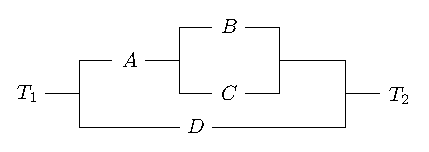
\includegraphics[height=20mm]{vezje.eps}
\caption{Primer vezja s štirimi stikali}\label{fig:vezje}
\end{center}
\end{figure}

Recimo, da imamo tako vezje in da vemo, katera stikala so odprta in katera zaprta.
Zanima nas, ali je celotno vezje ``zaprto"~(tj.,~skozenj teče tok) ali ``odprto"~(če
tok ne teče).


Poglejmo si dve zelo preprosti vezji:

(1) {\em zaporedno vezani stikali:}

\begin{figure}[h!]
\begin{center}
\includegraphics[height=5mm]{vezje-zaporedno.eps}\label{fig:vezje-zap}
\end{center}
\end{figure}

Zaporedno vezje je zaprto natanko tedaj, kadar sta obe stikali zaprti: {\bf konjunkcija}.

(2) {\em vzporedno vezani stikali:}

\begin{figure}[h!]
\begin{center}
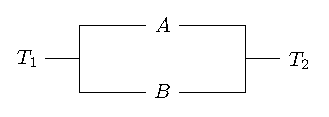
\includegraphics[height=20mm]{vezje-vzporedno.eps}\label{fig:vezje-vzp}
\end{center}
\end{figure}

Vzporedno vezje je zaprto natanko tedaj, kadar je vsaj eno stikalo zaprto:
{\bf disjunkcija}.

\medskip
Vsakemu takemu vezju ustreza neka logična izjava, sestavljena iz izjav, ki ustrezajo stikalom.

\medskip
Obratno: če omogočamo {\em identična} in {\em obratna} stikala, potem lahko
vsako sestavljeno izjavo predstavimo z vezjem!

Identični stikali sta taki stikali, ki sta bodisi hkrati odprti ali hkrati zaprti.

Obratni stikali sta taki stikali, da je natanko eno od njiju odprto.

\medskip
Zveza med vezji in izjavami:
{\em vezje je zaprto natanko tedaj, ko je ustrezna izjava pravilna, in odprto sicer.}

\medskip
\zgled
Vzemimo izjavo $$(A\sledi B) \inn (B\sledi C) \inn (\neg A \ali C)$$
V poglavju $1.2.$ smo izračunali pravilnostno tabelo te izjave:
$$\begin{tabular}{c|c|c|c|c}
  \hline
  % after \\: \hline or \cline{col1-col2} \cline{col3-col4} ...
   & $A$ & $B$ & $C$&$(A\sledi B) \inn (B\sledi C) \inn (\neg A \ali C)$\\
  \hline
  1. & 1& 1& 1 & 1 \\
  2. & 1& 1& 0 & 0 \\
  3. & 1& 0& 1 & 0 \\
  4. & 1& 0& 0 & 0 \\
  5. & 0& 1& 1 & 1 \\
  6. & 0& 1& 0 & 0 \\
  7. & 0& 0& 1 & 1 \\
  8. & 0& 0& 0 & 1 \\
\end{tabular}$$
V prejšnjem podpoglavju smo zapisali to izjavo v izbrani disjunktivni obliki kot:
$$(A\inn B\inn C) \ali (\neg A\inn B\inn C)\ali (\neg A\inn \neg B\inn C)\ali (\neg A\inn \neg B\inn \neg C)\,.$$

Tej obliki ustreza naslednje vezje:
\begin{figure}[h!]
\begin{center}
\includegraphics[height=35mm]{vezje-DNO.eps}\label{fig:vezje-DNO}
\end{center}
\end{figure}

Izbrani konjunktivni obliki
$$(\neg A\ali\neg B \ali C )\inn (\neg A\ali B \ali \neg C)\inn
(\neg A\ali B \ali C )\inn (A\ali \neg B \ali C)$$
pa ustreza vezje
\begin{figure}[h]
\begin{center}
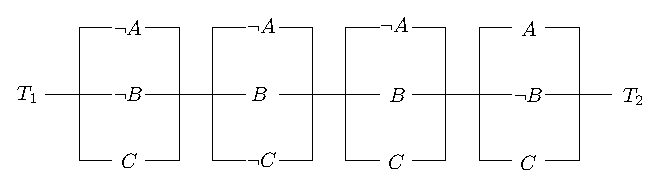
\includegraphics[height=20mm]{vezje-KNO.eps}\label{fig:vezje-KNO}
\end{center}
\end{figure}

Vidimo, da dani izjavi ustreza več preklopnih vezij.
Pri dejanski konstrukciji vezij, ki simulirajo dano izjavo, je torej
utemeljena zahteva, da naj bo vezje čimbolj enostavno, da naj ustreza določenim
predpisom itd.~(s tem se tu ne bomo ukvarjali).
\kz

\zgled
Dano je naslednje preklopno vezje:

\begin{figure}[h!]
\begin{center}
\includegraphics[height=35mm]{vezje2.eps}\label{fig:vezje2}
\end{center}
\end{figure}

{\em Pri katerih položajih stikal je vezje zaprto?} Problem rešimo z logiko.

Prirejena sestavljena izjava, recimo ji $D$, je:
$$(A \inn B\ali \neg C)\ali (\neg A \inn B)\ali (A \ali \neg C \inn \neg A)\,.$$
Njena pravilnostna tabela pa je:
$$\begin{tabular}{c|c|c|c|c|c|c|c}
  \hline
  % after \\: \hline or \cline{col1-col2} \cline{col3-col4} ...
   & $A$ & $B$ & $C$ & $A \inn B\ali \neg C$ & $\neg A \inn B$ & $A \ali \neg C \inn \neg A$ & $D$\\
  \hline
  1. & 1 & 1 & 1 & 1 & 0 & 0 & 1\\
  2. & 1 & 1 & 0 & 1 & 0 & 0 & 1\\
  3. & 1 & 0 & 1 & 0 & 0 & 0 & 0\\
  4. & 1 & 0 & 0 & 1 & 0 & 0 & 1\\
  5. & 0 & 1 & 1 & 0 & 1 & 0 & 1\\
  6. & 0 & 1 & 0 & 0 & 1 & 1 & 1\\
  7. & 0 & 0 & 1 & 0 & 0 & 0 & 0\\
  8. & 0 & 0 & 0 & 0 & 0 & 1 & 1\\
\end{tabular}$$
Vidimo, da je vezje odprto natanko takrat, ko je stikalo $B$ odprto, $C$ pa zaprto,
in zaprto v vseh drugih primerih.

Torej bi vezje lahko zamenjali tudi z naslednjim preprostejšim vezjem:
\begin{figure}[h!]
\begin{center}
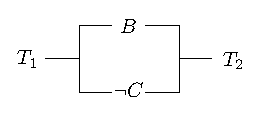
\includegraphics[height=15mm]{vezje3.eps}\label{fig:vezje3}
\end{center}
\end{figure}

Do istega rezultata lahko pridemo tudi po logični poti:

Iz pravilnostne tabele razberemo izbrano konjunktivno obliko izjave $D$
$$(\neg A \ali B \ali \neg C) \inn (A \ali B\ali \neg C)\,.$$
zaradi distributivnosti je ta izjava ekvivalentna izjavi
$$(\neg A \inn  A) \ali (B\ali \neg C)$$
ker pa je konjunkcija $\neg A \inn A$ vselej nepravilna, je ta izjava ekvivalentna izjavi
$B\ali \neg C\,.$

\kz

\medskip
Zaključimo poglavje o vezjih še z enim zgledom bolj praktične narave.

\medskip
\zgled
Imamo odbor 3 poslancev, ki glasujejo o posameznih predlogih po določenem volilnem načelu.
Konstruirati je treba tako preklopno vezje, ki
bo nemudoma sporočilo, ali je predlog sprejet ali ne.

Oglejmo si dve možni volilni načeli:

(a) načelo enostavne večine

(b) načelo enostavne večine, pri čemer ima poslanec $A$ pravico veta

Pravilnostna tabela veli:
$$\begin{tabular}{c|c|c|c|c}
  \hline
  % after \\: \hline or \cline{col1-col2} \cline{col3-col4} ...
$A$ & $B$ & $C$  & $(a)$ & (b)\\
  \hline
1 & 1 & 1 & 1  & 1  \\
1 & 1 & 0 & 1  & 1  \\
1 & 0 & 1 & 1  & 1  \\
1 & 0 & 0 & 0  & 0  \\
0 & 1 & 1 & 1  & 0  \\
0 & 1 & 0 & 0  & 0  \\
0 & 0 & 1 & 0  & 0  \\
0 & 0 & 0 & 0  & 0  \\
\end{tabular}$$
Če se odločimo za izbrano disjunktivno obliko, potem se zaželena izjava v primeru (a) glasi
$$(A\inn B\inn C)\ali (A\inn B\inn \neg C)\ali (A\inn \neg B\inn C)\ali (\neg A\inn B\inn C)$$
v primeru (b) pa
$$(A\inn B\inn C)\ali (A\inn B\inn \neg C)\ali (A\inn \neg B\inn C)\,.$$
Ustrezni vezji pa sta:

(a)
\begin{figure}[h!]
\begin{center}
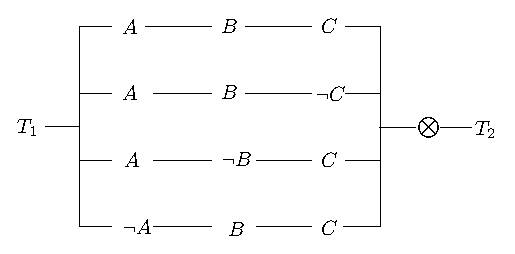
\includegraphics[height=30mm]{vezje-poslanci-1.eps}\label{fig:vezje-poslanci-1}
\end{center}
\end{figure}

(b)
\begin{figure}[h!]
\begin{center}
\includegraphics[height=20mm]{vezje-poslanci-2.eps}\label{fig:vezje-poslanci-2}
\end{center}
\end{figure}

\kz

{\bf Domača naloga:} Sestavite vezje, prirejeno izjavi
$$(A\sledi B) \ali (\neg B\sledi C) \ali (A \cee C)\,.$$



\subsection{Logične implikacije}

{\em Logična implikacija} je tavtologija, pri kateri je glavna povezava implikacija.

\iftoggle{long}{\komentar{Izpuščeno: OD TU}}

\iftoggle{long}{
{\color{blue}
Če je $B\sledi C$ tavtologija, potem je podprostor pravilnosti antecedensa (tj., izjave $B$) vsebovan v podprostoru pravilnosti konsekvensa (tj., izjave $C$). In obratno, če je podprostor pravilnosti antecedensa vsebovan v podprostoru pravilnosti konsekvensa, potem je
je $B\sledi C$ tavtologija.

\smallskip
{\bf Domača naloga:} Dokažite trditev, da je $B\sledi C$ tavtologija če in samo če je podprostor pravilnosti antecedensa vsebovan v podprostoru pravilnosti konsekvensa.
}\\
}

\iftoggle{long}{\komentar{Izpuščeno: DO TU}\\}

\bigskip
Veljajo naslednje resnice o logičnih implikacijah:
\begin{enumerate}
  \item Če je antecedens tavtologija, mora biti tudi konsekvens tavtologija.
  \item Če je konsekvens protislovje, mora biti tudi antecedens protislovje.
  \item Če je konsekvens tavtologija, je lahko antecedens katerakoli izjava.
  \item Če je antecedens protislovje, je lahko konsekvens katerakoli izjava.
  \item Vsaka izjava logično implicira samo sebe.
  \item Vsaka izjava, ki logično implicira hkrati kakšno izjavo $A$ in njeno negacijo $\neg A$, mora biti protislovje.
  \item Izjava, ki logično implicira svojo negacijo, je protislovje.
\end{enumerate}

\medskip
\iftoggle{long}{
{\color{blue}
Zgled logične implikacije:
$$A \sledi B \sledi (A\inn C \sledi B\inn C)\,.$$
Dokažimo jo. Ta implikacija bi bila nepravilna le pri takem določilu, pri katerem bi bila izjava
$A \sledi B$ pravilna, izjava $A\inn C \sledi B\inn C$ pa nepravilna. To je po definiciji implikacije res samo, če sta izjavi $A\inn C$ pravilni, izjava $B$ pa nepravilna.
V tem primeru pa je implikacija $A \sledi B$ nepravilna, kar je v nasprotju s predpostavko, da je
pravilna. Torej ne obstaja tako določilo, za katero bi bila izjava  $A \sledi B$ pravilna, izjava $A\inn C \sledi B\inn C$ pa nepravilna. Implikacija je res tavtologija.

\medskip
Logične implikacije z majhnim številom osnovnih izjav lahko dokažemo tudi z uporabo pravilnostnih tabel.

\medskip
Na vajah boste spoznali in dokazali številne druge logične implikacije.
}}
{
Zgled logične implikacije:
$$A \sledi B \sledi (A\inn C \sledi B\inn C)\,.$$
Dokažimo jo. Ta implikacija bi bila nepravilna le pri takem določilu, pri katerem bi bila izjava
$A \sledi B$ pravilna, izjava $A\inn C \sledi B\inn C$ pa nepravilna. To je po definiciji implikacije res samo, če sta izjavi $A\inn C$ pravilni, izjava $B$ pa nepravilna.
V tem primeru pa je implikacija $A \sledi B$ nepravilna, kar je v nasprotju s predpostavko, da je
pravilna. Torej ne obstaja tako določilo, za katero bi bila izjava  $A \sledi B$ pravilna, izjava $A\inn C \sledi B\inn C$ pa nepravilna. Implikacija je res tavtologija.

\medskip
Na vajah boste spoznali in dokazali številne druge logične implikacije.
}

\subsubsection*{Nekaj poglavitnih logičnih implikacij}

\begin{enumerate}
  \item $A \inn (A \sledi B) \sledi B$
  \item $\neg B \inn (A \sledi B) \sledi \neg A$
  \item $\neg A \inn (A \ali B) \sledi B$
  \item $A \inn B \sledi A$
  \item $A \sledi A\ali B$
  \item $A \inn \neg A\sledi B$
  \item $(A \sledi B) \inn (B \sledi C) \sledi (A\sledi C)$
  \item $(A \sledi B) \sledi ((C \sledi A) \sledi (C\sledi B))$
  \item $(A \sledi B) \sledi ((B \sledi C) \sledi (A\sledi C))$
  \item $(A \sledi B) \sledi (A\inn C \sledi B\inn C)$
  \item $(A \sledi B) \sledi (A\ali C \sledi B\ali C)$
  \item $(A \cee B) \inn (B\cee C) \sledi (A\cee C)$
  \item $(A \cee B) \sledi (A\sledi B)$
  \item $(A \cee B) \sledi (B\sledi A)$
  \item $A \inn (A \cee B) \sledi B$
  \item $\neg A \inn (A \cee B) \sledi \neg B$
  \item $B\sledi (A\cee A \inn B)$
  \item $\neg B\sledi (A\cee A \ali B)$
  \item $(A\sledi (B\inn \neg B)) \sledi \neg A$
\end{enumerate}

Za vajo se prepričajte o veljavnosti teh logičnih implikacij. Namesto pravilnostnih tabel lahko uporabite tole metodo:  {\em Izhajamo iz definicije implikacije in poskušamo konstruirati tako določilo, za katero bi bila implikacija nepravilna. Potem se mora seveda izkazati, da takega določila ni.}

\bigskip
\zgled
Dokažimo 10. logično implikacijo s seznama:
$$A \sledi B \sledi (A\inn C \sledi B\inn C)$$
Ta implikacija bi bila nepravilna le pri takem določilu, pri katerem bi bila izjava
$A \sledi B$ pravilna, izjava $A\inn C \sledi B\inn C$ pa nepravilna. To je po definiciji implikacije res samo, če sta izjavi $A\inn C$ pravilni, izjava $B$ pa nepravilna.
V tem primeru pa je implikacija $A \sledi B$ nepravilna, kar je v nasprotju s predpostavko, da je
pravilna. Torej ne obstaja tako določilo, za katero bi bila izjava  $A \sledi B$ pravilna, izjava $A\inn C \sledi B\inn C$ pa nepravilna. Implikacija 10.~je res tavtologija.\kz



\medskip

\iftoggle{long}{\komentar{Izpuščeno: OD TU}}

\iftoggle{long}{
{\color{blue}

{\bf Nekaj komentarjev k implikacijam:}

(1.) Iz pravilnosti antecedensa in pravilnosti implikacije sklepamo na pravilnost konsekvensa. To je t.i.~{\em zakon osamitve}.
\begin{itemize}
  \item V klasični logiki so imenovali ta sklep {\em mešani hipotetični silogizem} in sicer {\em načina ponendo ponens} (lat. način, ki potrjuje s potrditvijo)
\end{itemize}

\zgled
Če je danes sreda, bom šel na predavanja.

Danes je sreda.

Sklep: Šel bom na predavanja.\kz

(2.) {\em mešani hipotetični silogizem} {\em načina tollendo tollens} (lat. način, ki zanika z zanikanjem)

{\bf Zgleda:}

1. Kjer je dim, je tudi ogenj.

Tu ni ognja.

Sklep: Tu ni dima.

2. Dobro živi, komur je malo zadosti.

Pohlepni ne živi dobro.

Sklep: Pohlepnemu malo ni zadosti.


(3.) {\em disjunktivni silogizem} {\em načina tollendo ponens}
(lat. način, ki potrjuje z zanikanjem)

{\bf Zgled:}

Koper je država ali pa je mesto.

Koper ni država.

Sklep: Koper je mesto.

(4.) Zakon poenostavitve.

(5.) Zakon dodajanja.

(6.) Iz protislovja lahko izpeljemo katerokoli izjavo.

(7.) Tranzitivnost implikacije (t.i.~{\em čisti hipotetični silogizem}).

(12.) Tranzitivnost ekvivalence.

(19.) Zakon o absurdu.
}
\\}

\iftoggle{long}{\komentar{Izpuščeno: DO TU.}\\}

\newpage 

\subsection{Načini dokazovanja}

Logične implikacije uporabljamo pri dokazovanju novih trditev iz aksiomov in že dokazanih trditev.
Poglejmo si nekaj načinov dokazovanja.

\subsubsection*{1)~Direktni dokaz implikacije $A \sledi  B$}

Dokazujemo logično implikacijo $A \sledi  B$.
Predpostavimo, da je $A$ pravilna izjava in direktno izpeljemo pravilnost izjave $B$.

\medskip

\zgled

{\it Če je $n$ liho naravno število, je tudi $n^2$ liho število.}

\medskip \noindent{\bf Dokaz.}
Naj bo $n$ liho naravno število. Tedaj ga lahko zapišemo kot $n = 2k-1$, kjer je $k$ naravno število. Sledi $n^2 = (2k-1)^2 = 4k^2-4k+1 = 2(2k^2-2k)+1$, torej je $n^2$ liho število.\qed

\medskip

\begin{center}
\fbox{\parbox{0.5\linewidth}{\noindent
{\bf Direktni dokaz implikacije $A \sledi  B$}

{\bf Dokaz:}

Predpostavimo $A$.

~~~~$\vdots$

Torej, $B$.

Sledi $A \sledi  B$.\hspace{-2cm}\qed
}}
\end{center}

\subsubsection*{2)~Indirektni dokaz implikacije $A \sledi  B$}

Dokazujemo pravilnost logične implikacije $A \sledi  B$.
Včasih se izkaže, da je ugodneje
direktno dokazovati ekvivalentno implikacijo $\neg B \sledi \neg A$.

\medskip
\zgled

{\it Če je $n^2$ sodo število, je $n$ sodo število.}

\medskip \noindent{\bf Dokaz.}
Izjava je ekvivalentna implikaciji:

Če je $n$ število, ki ni sodo, je $n^2$ število, ki ni sodo.

Ekvivalentno: Če je $n$ liho število, je $n^2$ liho število.

To pa smo že dokazali.\qed

\medskip

\begin{center}
\fbox{\parbox{0.5\linewidth}{\noindent
{\bf Indirektni dokaz implikacije $A \sledi  B$}

{\bf Dokaz:}

Predpostavimo $\neg B$.

~~~~$\vdots$

Torej, $\neg A$.

Sledi $\neg B \sledi  \neg A$.

Posledično $A \sledi  B$.\hspace{-2cm}\qed
}}
\end{center}

\subsubsection*{3)~Dokaz izjave $A$ s protislovjem}

Želimo dokazati pravilnost izjave $A$. Predpostavimo, da je $A$ nepravilna in pokažemo, da vodi ta predpostavka v protislovje (ki ga označimo s $\perp$). S tem smo pokazali pravilnost izjave $\neg A \sledi \perp$. Ta izjava pa je pravilna le, če je izjava $\neg A$ nepravilna, torej je $A$ pravilna.

\medskip
\zgled

{\it Število $\sqrt 2$ ni racionalno.}

\medskip \noindent{\bf Dokaz.} Predpostavimo, da je $\sqrt 2$ racionalno število. Tedaj ga lahko zapišemo kot $\sqrt 2 = p/q$, kjer sta $p$ in $q$ tuji si naravni števili.

Sledi

$2 = p^2/q^2$.

$p^2 = 2q^2$.

Torej je $p^2$ sodo število. Sledi (po prej dokazanem), da je $p$ sodo število.

Pišimo $p = 2m$, kjer je $m$ naravno število.

Dobimo

$4m^2 = 2q^2$.

Sledi
$2m^2 = q^2$.

Torej je tudi $q$ sodo število. To pa je protislovje. (Predpostavili smo, da sta $p$ in $q$ tuji si števili in dokazali, da sta obe deljivi z 2, torej da si nista tuji.)\qed

\medskip
\begin{center}
\fbox{\parbox{0.7\linewidth}{\noindent
{\bf Dokaz izjave $A$ s protislovjem}

{\bf Dokaz:}

Predpostavimo $\neg A$.

~~~~$\vdots$

Torej, $B$.

~~~~$\vdots$

Torej, $\neg B$.

Sledi, da je pravilna tudi izjava $B\inn \neg B$, ta pa je protislovje.

Posledično $A$.\hspace{-2cm}\qed
}}
\end{center}


\subsubsection*{4)~Dokaz ekvivalence $A\cee B$ v dveh delih}

Želimo dokazati pravilnost logične ekvivalence $A\cee B$.
Dokažemo vsako od obeh implikacij.

Za dokazovanje obeh delov lahko uporabimo različne metode.
Pogosto je dokaz implikacije v eno smer lažji od dokaza v drugo smer.

\zgled

{\it Pozitivno celo število $p>1$ je praštevilo natanko tedaj, ko ne obstaja tako naravno število
$n$, večje od $1$ in manjše ali enako $\sqrt{p}$, ki deli $p$.}

\medskip \noindent{\bf Dokaz.}

(i) Dokazujemo indirektno. Predpostavimo, da obstaja tako naravno število
$n$, večje od $1$ in manjše ali enako $\sqrt{p}$, ki deli $p$. Torej je $n$ delitelj $p$, različen od
$1$ in $p$, in $p$ ni praštevilo.

(ii) Tudi tu dokazujemo indirektno. Predpostavimo, da $p$ ni praštevilo. Lahko ga torej zapišemo v obliki
$p = n_1\cdot n_2$, kjer sta $n_1$ in $n_2$ pozitivni celi števili, različni od $1$ in $p$.
Trdimo, da je vsaj eno od  števil $n_1$ in $n_2$ manjše ali enako $\sqrt{p}$.
Če to ne bi veljalo, bi imeli $n_1>\sqrt{p}$ in $n_2>\sqrt{p}$ in posledično
$p = n_1n_2>\sqrt{p}\cdot\sqrt{p} = p$, protislovje.
Naj bo torej $n$ tako število izmed $n_1$ in $n_2$, za katerega velja  $n\le \sqrt{p}$.
Število $n$ je tedaj naravno število, večje od $1$ in manjše ali enako $\sqrt{p}$, ki deli $p$.\qed

\medskip
\zgled

{\it Naj bosta $m$ in $n$ celi števili. Tedaj sta števili $m$ in $n$ iste parnosti natanko tedaj, ko je število $m^2 + n^2$ sodo.}

\medskip \noindent{\bf Dokaz.}

(i) Predpostavimo, da sta $m$ in $n$ iste parnosti. Obravnavamo dva primera.
\begin{enumerate}[(a)]
  \item Če sta $m$ in $n$ sodi števili, potem je $m = 2k$ in $n = 2j$ za neki celi števili $k$ in $j$.
  Sledi $m^2+n^2 = (2k)^2+(2j)^2 = 2(2k^2+2j^2)$, kar je sodo število.
  \item Če sta $m$ in $n$ lihi števili, potem je $m = 2k+1$ in $n = 2j+1$ za neki celi števili $k$ in $j$.
  Sledi $m^2+n^2 = (2k+1)^2+(2j+1)^2 = 2(2k^2+2k+2j^2+2j+1)$, kar je sodo število.
\end{enumerate}
V obeh primerih je $m^2+n^2$ sodo število.

(ii) Predpostavimo, da je $m^2+n^2$ sodo število. Spet obravnavamo dva primera.
\begin{enumerate}[(a)]
  \item Če je $m$ sodo število, potem je tudi $m^2$ sodo število. Torej, ker je $m^2+n^2$ sodo število in $m^2$ sodo število, je sodo tudi število
  $n^2 = (m^2+n^2)-m^2$. Od tod sledi, da je $n$ sodo.
  \item Če je $m$ liho število, potem je tudi $m^2$ liho število.
  Torej, ker je $m^2+n^2$ sodo število in $m^2$ liho število, je liho tudi število
  $n^2 = (m^2+n^2)-m^2$. Od tod sledi, da je $n$ liho.
  \end{enumerate}
V obeh primerih sta $m$ in $n$ iste parnosti.
\qed

Povzemimo:

\begin{center}
\fbox{\parbox{0.5\linewidth}{\noindent
{\bf Dokaz ekvivalence $A\cee B$ v dveh delih}

{\bf Dokaz:}

(i) Dokažemo $A\sledi B$.

(ii) Dokažemo $B\sledi A$.

Torej, $A\cee B$.\hspace{-2cm}\qed
}}
\end{center}

% predavanje 11. oktober (2h) konec
%\end{document}

\subsubsection*{5)~``Če in samo če'' dokaz $A\cee B$}

Pravilnost logične ekvivalence $A\cee B$ lahko dokažemo
z zaporedjem logično ekvivalentnih izjav. Začnemo z izjavo $A$ in
jo zamenjamo z zaporedjem ekvivalentnih izjav, ki se konča z izjavo $B$.

\medskip
\zgled

{\it Dan je trikotnik $T$ s stranicami dolžin $a$, $b$, $c$. S pomočjo kosinusnega izreka
dokaži, da je $T$ pravokotni trikotnik s hipotenuzo dolžine $c$ natanko tedaj, ko je $a^2+b^2 = c^2$.}

Kosinusni izrek: $a^2+b^2 = c^2+2ab \cos \gamma$, kjer je $\gamma$ kot med stranicama dolžin $a$ in $b$.

\medskip
\medskip \noindent{\bf Dokaz.}

Iz kosinusnega izreka sledi

$a^2+b^2 = c^2$~~~~če in samo če~~~~$2ab\cos \gamma = 0$

~~~~~~~~~~~~~~~~~~~~če in samo če~~~~$\cos \gamma = 0$

~~~~~~~~~~~~~~~~~~~~če in samo če~~~~$\gamma = 90^\circ$.

Torej je $a^2+b^2 = c^2$ natanko tedaj, ko je $T$ pravokotni trikotnik s hipotenuzo dolžine~$c$.
\qed

\medskip

%\newpage
Če imamo $n$ vmesnih izjav $C_1,\ldots, C_n$, ima dokaz naslednjo obliko:

\begin{center}
\fbox{\parbox{0.5\linewidth}{\noindent
{\bf ``Če in samo če'' dokaz $A\cee B$}

{\bf Dokaz:}

$A$~~če in samo če~~$C_1$

~~~~če in samo če~~$C_2$

~~~~$\ldots$

~~~~če in samo če~~$C_n$

~~~~če in samo če~~$B$.\hspace{-2cm}\qed
}}
\end{center}

\subsubsection*{6)~Analiza primerov}
Včasih nam pri dokazu pravilnosti izjave $A$ pomaga, če pregledamo vse primere, ter ugotovimo da je $B$ vedno pravilna.


\begin{center}
	\fbox{\parbox{0.6\linewidth}{\noindent
			{\bf Dokazovanje $A$ s pomočjo analize primerov.}
			
			{\bf Dokaz:}
			
			Primer 1: predpostavimo $B$
			
			~~~~$\ldots$
			
			~~~~$A$.
			
			Primer 2: predpostavimo $\neg B$
			
			~~~~$\ldots$
			
			~~~~$A$.\hspace{-2cm}\qed
	}}
\end{center}

% predavanja 24.10. ponovitev načinov dokazovanja
% analiza primerov..

\newpage
\subsection{Množice izjav}

Dane so atomarne izjave $A_1,\ldots, A_n$ (take, da v njih ne nastopa nobena logična povezava).

Koliko različnih izjav lahko sestavimo iz njih?

Zdi se, da neskončno mnogo! Vendar pa, za logiko sta dve izjavi isti, če sta logično ekvivalentni.

Izjav, ki med seboj niso logično ekvivalentne, pa je le končno mnogo.

Vsaka izjava, sestavljene iz $A_1,\ldots, A_n$, ima natanko $2^n$ različnih določil.
Izjava je enolično določena, brž ko so določene njene vrednosti za vsako od teh $2^n$ določil.

Vsako določilo ima vrednost 0 ali 1, neodvisno od drugih. Sledi, da je vseh možnih izjav
$2^{(2^n)}$.

\bigskip
Oglejmo si konstrukcijo vseh možnih izjav za $n = 1$ in $n=2$.

{\bf n = 1}

Imamo eno samo izjavo, $A$. Iz nje lahko sestavimo $2^{(2^1)} = 4$ izjave, $C_1,\ldots, C_4$.

$$\begin{tabular}{c|c|c|c|c}
  \hline
  % after \\: \hline or \cline{col1-col2} \cline{col3-col4} ...
$A$ & $C_1$ & $C_2$  & $C_3$ & $C_4$\\
  \hline
1 & 1 & 1 & 0  & 0  \\
0 & 1 & 0 & 1  & 0  \\
\end{tabular}$$

$C_1$ je tavtologija, npr.~$A\ali \neg A$.

$C_4$ je protislovje, npr.~$A\inn \neg A$.

Za $C_2$ lahko vzamemo kar $A$.

Za $C_3$ pa $\neg A$.


\bigskip
{\bf n = 2}

Imamo dve izjavi, $A$ in $B$. Iz njiju lahko sestavimo $2^{(2^2)} = 16$ izjav,
$C_1,\ldots, C_{16}$.

$$\begin{tabular}{c|c|c|c|c|c|c|c|c|c|c|c|c|c|c|c|c|c}
  \hline
  % after \\: \hline or \cline{col1-col2} \cline{col3-col4} ...
$A$ & $B$
& $C_1$ & $C_2$  & $C_3$ & $C_4$
& $C_5$ & $C_6$  & $C_7$ & $C_8$
& $C_9$ & $C_{10}$  & $C_{11}$ & $C_{12}$
& $C_{13}$ & $C_{14}$  & $C_{15}$ & $C_{16}$\\
  \hline
1 & 1 &   1 & 1 & 1 & 1 & 1 & 1 & 1 & 1 & 0 & 0 & 0 & 0 & 0 & 0 & 0 & 0\\
1 & 0 &   1 & 1 & 1 & 1 & 0 & 0 & 0 & 0 & 1 & 1 & 1 & 1 & 0 & 0 & 0 & 0\\
0 & 1 &   1 & 1 & 0 & 0 & 1 & 1 & 0 & 0 & 1 & 1 & 0 & 0 & 1 & 1 & 0 & 0\\
0 & 0 &   1 & 0 & 1 & 0 & 1 & 0 & 1 & 0 & 1 & 0 & 1 & 0 & 1 & 0 & 1 & 0\\
\end{tabular}$$

Seveda je $C_1$ je tavtologija, npr.~$A\ali \neg A$ in
$C_{16}$ protislovje $A\inn \neg A$.

Ker so izjave $C_2$, $C_3$, $C_5$ in $C_9$ nepravilne le pri enem določilu, bomo v teh primerih izbrali
izbrano konjunktivno obliko:
\begin{itemize}
  \item $C_2 = A\ali B$
  \item $C_3 = A\ali \neg B$
  \item $C_5 = \neg A\ali B$
  \item $C_8 = \neg A\ali \neg B$
\end{itemize}
Podobno za izjave $C_{8}$, $C_{12}$, $C_{14}$ in $C_{15}$ izrazimo s pomočjo izbrane disjunktivne oblike:
\begin{itemize}
  \item $C_8 = A\inn B$
  \item $C_{12} = A\inn\neg B$
  \item $C_{14} = \neg A\inn B$
  \item $C_{15} = \neg A\inn\neg B$
\end{itemize}
Vse preostale izjave pa so pravilne pri dveh določilih in prav tako nepravilne pri dveh določilih.

Za $C_4$ vzamemo $$(A\inn B) \ali (A\inn \neg B)\,,$$
kar je ekvivalentno
$$A\inn (B \ali \neg B)$$
in ker je disjunkcija $B \ali \neg B$ vedno pravilna izjava, je torej izjava $C_4$ ekvivalentna z izjavo $A$.

Podobno se prepričamo, da je:
\begin{itemize}
  \item  izjava $C_6$ ekvivalentna z izjavo $B$,
  \item  izjava $C_{11}$ ekvivalentna z izjavo $\neg B$,
  \item  izjava $C_{13}$ ekvivalentna z izjavo $\neg A$.
\end{itemize}
Za $C_7$ pišimo
$$(A\inn B) \ali (\neg A\ali \neg B)\,,$$
kar je ekvivalentno z
$$A\cee B\,.$$
Podobno pa lahko za $C_{10}$ vzamemo ekvivalenco
$$A\cee \neg B\,.$$
\qed
\subsection{Pravila sklepanja}
Kako pa pokažemo pravilnost sklepa? Zapis
pravilnostne tabele in preverjanje vseh naborov je časovno potraten postopek. Precej
rajši bi imeli kratko izpeljavo, v kateri bi izvajali relativno enostavne, majhne korake
proti cilju.
Majhne, enostavne sklepe, ki jih bomo potrebovali za dokazovanje pravilnosti sklepov,
imenujemo pravila sklepanja.

\begin{tabular}{|c|c|c|}
	\hline 
	ime & predpostavke & sklep\\
	\hline 
	\hline 
	modus ponens & $A,A\Rightarrow B$ & $B$\\
	\hline 
	modus tollens & $A\Rightarrow B,\neg B$ & $\neg A$\\
	\hline 
	hipoteti\v{c}ni silogizem & $A\Rightarrow B,B\Rightarrow C$ & $A\Rightarrow C$\\
	\hline 
	disjunktivni silogizem & $A\vee B,\neg A$ & $B$\\
	\hline 
	združitev  & $A,B$ & $A\wedge B$\\
	\hline 
	poenostavitev & $A\wedge B$ & $A$\\
	\hline 
	pridružitev & $A$ & $A\vee B$\\
	\hline 
\end{tabular}

{
\subsection{Izjave s predikati in kvantifikatorji}
}

Kvantifikatorji povedo, za koliko objektov neke vrste velja neka izjava.
Pri tem moramo povedati, katere vrste objekti nas zanimajo (npr.~elementi množic $\mathbb{N}$, $\mathbb{Z}$, $\mathbb{Q}$, $\mathbb{R}$, $\mathbb{C}$, itd.), pogosto pa je to že razvidno iz konteksta.

Naj bo $A(x)$ neka izjava, smiselna za vsak objekt $x$ iz domene pogovora.
\iftoggle{long}{
{\color{blue}Taki izjavi pravimo {\it predikat}.
Predikati oblike $A(x)$ so enomestni. Poznamo pa tudi dvo- in večmestne predikate, npr.~$A(x,y)$, $P(x_1,x_2,x_3)$ ipd.}
}
{Taki izjavi pravimo {\it predikat}. Predikati oblike $A(x)$ so enomestni. Poznamo pa tudi dvo- in večmestne predikate, npr.~$A(x,y)$, $P(x_1,x_2,x_3)$ ipd.}

Za zapis izjav s kvantifikatorji bomo uporabljali naslednje oznake:
\begin{itemize}
  \item
  $(\forall x) A(x)$: to je izjava, ki je pravilna natanko tedaj, ko je za vsak $x$ izjava $A(x)$ pravilna

$\forall$ je t.i.~{\it univerzalni kvantifikator}
  \item
  $(\exists  x) A(x)$: to je izjava, ki je pravilna natanko tedaj, ko obstaja vsaj en $x$, za katerega je izjava $A(x)$ pravilna

$\exists$ je t.i.~{\it eksistencialni kvantifikator}

  \item
  $(\exists!  x) A(x)$: to je izjava, ki je pravilna natanko tedaj, ko obstaja {\bf natanko en} $x$, za katerega je izjava $A(x)$ pravilna

Ekvivalentno: $(\exists x)A(x) \inn (\forall y)(\forall z)(A(y) \inn A(z) \sledi y = z)$
\end{itemize}

\zgled
Zadnjič smo dokazali izjavo {\it Če je $n$ liho naravno število, je tudi $n^2$ liho število.}
To pomeni: za vsako naravno število $n$ velja, da če je liho, potem je tudi $n^2$ liho število.
To lahko zapišemo kot $(\forall n)A(n)$, kjer je $A(n)$ izjava ``Če je $n$ liho število, potem je tudi $n^2$ liho število."
\kz

\medskip
\begin{sloppypar}
\zgled
Dana je izjava ``Vsa jabolka so okusna.''
Kako bi to izjavo zapisali s predikati in kvantifikatorji?

Uporabimo $\forall$, a kako?

Če se omejimo le na objekte, ki so jabolka, potem zapišemo $(\forall x)(x$ je okusen).

Če pa je $x$ lahko poljubno sadje, potem moramo uporabiti dve izjavi:

$A(x)$: $x$ je jabolko

 in

$B(x)$: $x$ je okusen

Kako pa zapišemo izjavo vsi $A(x)$ so $B(x)$? Kot $(\forall x)(A(x)\inn B(x))$
ali kot $(\forall x)(A(x) \sledi B(x))$?
Prva izjava bi pomenila, da je vsako sadje okusno jabolko, tega pa ne želimo trditi. Pravilen je drugi zapis.
\kz
\end{sloppypar}

\medskip
\zgled
Dana je izjava ``Nekatera jabolka so okusna.'' Kako bi pa to izjavo zapisali s kvantifikatorji, pri čemer kot objekte upoštevamo vse vrste sadja?
Naj bo spet

$A(x)$: $x$ je jabolko
 in
$B(x)$: $x$ je okusen

Bomo zapisali $(\exists x)(A(x)\inn B(x))$ ali $(\exists x)(A(x) \sledi B(x))$?

Prva izjava pomeni, da obstaja sadje, ki je okusno jabolko, in to je pravilen zapis.
Druga izjava pa trdi, da za vsako sadje velja, da če je jabolko, potem je okusno. Ta izjava pa ne zagotavlja obstoja jabolka;
pravilna je v vsakem kontekstu, kjer obstaja objekt, ki ni jabolko ali pa je okusno. Tega pa ne želimo trditi.
\kz

\medskip
Povzemimo:

{\it Izjavo oblike ``vsi $A(x)$ so $B(x)$'' zapišemo kot $(\forall x)(A(x)\sledi B(x))$.

Izjavo oblike ``nekateri $A(x)$ so $B(x)$'' pa kot $(\exists x)(A(x)\inn B(x))$.}

\medskip

\medskip
\noindent{\bf Še nekaj zgledov izjav s kvantifikatorji:}

\iftoggle{long}{
{\color{blue}Naj bo domena pogovora množica naravnih števil. Tedaj so naslednje izjave s kvantifikatorji smiselne:}
\begin{itemize}
  \item $(\forall$ $n)$ ($n$ je deljiv z 2).
  \item
$(\exists n)$ ($n$ je deljiv z 2).
  \item
$(\exists !n)$ ($n$ je najmanjše naravno število).
\end{itemize}

Kako bi zapisali zgornje izjave, če bi bila domena pogovora množica realnih števil z uporabo predikata
$N(n):$ ``$n$ je naravno število''?
\begin{itemize}
  \item $(\forall$ $n)$ ($N(n)\sledi n$ je deljiv z 2).
  \item
$(\exists n)$ ($N(n)\inn n$ je deljiv z 2).
  \item
$(\exists !n)$ ($N(n)\inn n$ je najmanjše naravno število).
\end{itemize}

\medskip
}
{Naj bo domena pogovora množica naravnih števil. Tedaj so naslednje izjave s kvantifikatorji smiselne:
\begin{itemize}
  \item $(\forall$ $n)$ ($n$ je deljiv z 2).
  \item
$(\exists n)$ ($n$ je deljiv z 2).
  \item
$(\exists !n)$ ($n$ je najmanjše naravno število).
\end{itemize}
Kako bi zapisali zgornje izjave, če bi bila domena pogovora množica realnih števil z uporabo predikata
$N(n):$ ``$n$ je naravno število''?
\begin{itemize}
  \item $(\forall$ $n)$ ($N(n)\sledi n$ je deljiv z 2).
  \item
$(\exists n)$ ($N(n)\inn n$ je deljiv z 2).
  \item
$(\exists !n)$ ($N(n)\inn n$ je najmanjše naravno število).
\end{itemize}
}


\subsubsection{Negacije izjav s kvantifikatorji}

{\bf Negacija $\forall$}
$$\neg (\forall x)A(x) \cee  (\exists x) (\neg A(x))$$

\medskip
\zgled

$B$: Vsak državljan Slovenije je rjavolas.

$\neg B$: Ni res, da je vsak državljan Slovenije rjavolas.

Ekvivalentno: Obstaja vsaj en državljan Slovenije, ki ni rjavolas.\kz

\medskip

\noindent{\bf Negacija $\exists$}
$$\neg  (\exists x)A(x) \cee (\forall x) \neg A(x)$$

\medskip
\zgled

$B$: V škatli obstaja rdeča kroglica.

$\neg B$: Ni res, da obstaja v škatli rdeča kroglica.

Ekvivalentno: Za vse kroglice v škatli velja, da niso rdeče.\kz


%VAJE:
%\zgled
%
%Zapiši negacijo izjave $(\exists ! x)A(x)$.
%
%$(\exists ! x)A(x)\cee (\exists x)A(x) \inn (\forall y)(\forall z)(A(y) \inn A(z) \sledi y = z)$
%
%Sledi:
%
%$\neg (\exists ! x)A(x)\cee \neg \left((\exists x)A(x) \inn (\forall y)(\forall z)(A(y) \inn A(z) \sledi y = z)\right)$
%
%$\cee \neg (\exists x)A(x) \ali \neg (\forall y)(\forall z)(A(y) \inn A(z) \sledi y = z)$
%
%$\cee (\forall x)\neg A(x) \ali (\exists y)\neg \left((\forall z)(A(y) \inn A(z) \sledi y = z)\right)$
%
%$\cee (\forall x)\neg A(x) \ali (\exists y)(\exists z)\neg (A(y) \inn A(z) \sledi y = z)$
%
%$\cee (\forall x)\neg A(x) \ali (\exists y)(\exists z)(A(y) \inn A(z) \inn y \neq z)$
%\kz
%
%\medskip
%\zgled
%
%$B$: Obstaja natanko eno praštevilo.
%
%$\neg B$: Ni res, da obstaja natanko eno praštevilo.
%
%Ekvivalentno: Nobeno število ni praštevilo ali obstajata vsaj dve praštevili.\kz
%
%\medskip
\zgled

Naj $P(x)$ označuje izjavo ``$x$ je praštevilo".

Za vsako naravno število $x$ obstaja naravno število $y$, večje od $x$, ki je praštevilo:
  $(\forall x)(\exists y)(y>x\inn P(y))$.

  Negacija:

  $\neg (\forall x)(\exists y)(y>x\inn P(y)) \cee(\exists  x)\neg (\exists y)(y>x\inn P(y))$

  $\cee(\exists  x)(\forall  y)\neg (y>x\inn P(y))\cee(\exists  x)(\forall  y)(y\le x\ali \neg P(y))\,.$\kz

\bigskip
\zgled
Zapišimo negacijo izjave
  $(\forall x)(\exists y)(y<x)\,.$

  $\neg(\forall x)(\exists y)(y<x)$

  $\cee (\exists x)(\neg(\exists y)(y<x))$

  $\cee (\exists x)(\forall y)\neg(y<x)$

  $\cee (\exists x)(\forall y)(y\ge x)$
  \kz

\begin{itemize}
  \item Ali je izjava pravilna v realnih številih?

  $(\forall x)(\exists y)(y<x)$

  Da, izjava je pravilna!

  \item Ali je izjava pravilna v naravnih številih?
  $(\forall x)(\exists y)(y<x)$

Ne, pravilna je njena negacija:
$(\exists x)(\forall y)(y\ge x)\,,$
obstaja namreč najmanjše naravno število.
\end{itemize}

{\bf Domača naloga:}
%\zgled

Ali je naslednja izjava pravilna?

Obstaja realno število $x$, za katerega velja $\frac{1}{1+x^2}>1$.

%$(\exists x) (\frac{1}{1+x^2} > 1)$
%
%Izjava ni pravilna. Prepričamo se namreč lahko v pravilnost njene negacije:
%
%$\neg (\exists x) (\frac{1}{1+x^2} > 1)$
%
%$\cee (\forall x) \neg (\frac{1}{1+x^2} > 1)$
%
%$\cee (\forall x) (\frac{1}{1+x^2} \le  1)$
%
%$\cee (\forall x) (1 \le  1+x^2)$
%
%$\cee (\forall x) (0 \le  x^2)$
%
%Torej:
%$\neg  \left(\exists \textrm{ realno število }x: \frac{1}{x^2+1}>1\right)$\kz


\subsubsection{Dokazovanje izjav s kvantifikatorji}

Poglejmo si nekaj načinov dokazovanja izjav s kvantifikatorji.

\subsubsection*{1)~Direktni dokaz izjave $(\forall x)A(x)$}

Dokazujemo trditev oblike $(\forall x)A(x)$.  Pokazati moramo torej, da je izjava $A(x)$
pravilna za vsak objekt $x$ iz domene pogovora.

\medskip
\zgled
{\it Dokaži, da za vsako naravno število $n$ velja $4n^2-4n+1\ge 0$.
}

\medskip \noindent{\bf Dokaz.}

{\it Trditev je oblike $(\forall x)A(x)$, kjer preučujemo naravna števila, $\mathbb{N}$, in je $A(x)$ izjava ``$4x^2 -4x+1 \ge 0$''.}

Naj bo $n$ poljubno naravno število. Zapišimo $4n^2 -4n+1 = (2n-1)^2$.
Kvadrat poljubnega realnega števila je nenegativno število.
Torej je $4n^2 -4n+1\ge 0$. Ker je bilo število $n$ poljubno, smo pokazali, da velja
 $4n^2-4n+1\ge 0$ za vsa naravna števila.
\qed

\medskip
\begin{center}
\fbox{\parbox{0.85\linewidth}{\noindent
{\bf Direktni dokaz izjave $(\forall x)A(x)$}

\medskip {\bf Dokaz:}

Naj bo $x$ poljuben objekt iz domene pogovora. {\it (Katere vrste objektov preučujemo, mora biti zapisano v trditvi ali razvidno iz konteksta.)}

~~~~$\vdots$

Torej, $A(x)$ je pravilna izjava.

Ker je bil $x$ poljuben, je izjava $(\forall x)A(x)$ pravilna. \qed
}}
\end{center}


\subsubsection*{2)~Dokaz izjave $(\forall x)A(x)$ s protislovjem}

Za dokazovanje izjav oblike $(\forall x)A(x)$  pogosto uporabimo dokaz s protislovjem.

\medskip
\zgled
{\it Dokaži, da za vse $x\in (0,\pi/2)$ velja $\sin x+\cos x>1$.
}

\medskip \noindent{\bf Dokaz.}

{\it Trditev je oblike
$(\forall x)A(x)$, kjer je
%preučujemo elemente odprtega intervala $(0,\pi/2)$ in je
$A(x)$ izjava ``$0<x<\pi/2\sledi \sin x+\cos x>1$''.}

Predpostavimo, da je trditev napačna.
Tedaj obstaja neko realno število $t$, za katerega je $0<t<\pi/2$ in $\sin t+\cos t\le 1$.
Ker sta funkciji $\sin x$ in $\cos x$ pozitivni za vse $x\in (0,\pi/2)$, velja $\sin t>0$ in $\cos t>0$.
Sledi:

$0<\sin t+\cos t \le 1$

$0<(\sin t+\cos t)^2 \le 1^2 = 1$

$0<\sin^2 t+2\sin t\cos t + \cos ^2t  \le 1$

$0<1+2\sin t\cos t \le 1$

$-1<2\sin t\cos t \le 0$

(Uporabili smo identiteto $\sin^2 t + \cos^2 t = 1$.)

Ampak $2\sin t\cos t\le 0$ je nemogoče, saj sta tako $\sin t$ kot $\cos t$ pozitivna.
Torej, če je $0<x<\pi/2$, potem je $\sin x+\cos x>1$.
\qed

\medskip
Ker je izjava $\neg(\forall x)A(x)$ ekvivalentna izjavi $(\exists x)\neg A(x)$, ima dokaz s protislovjem naslednjo obliko:

\begin{center}
\fbox{\parbox{0.85\linewidth}{\noindent
{\bf Dokaz izjave $(\forall x)A(x)$ s protislovjem}

\medskip {\bf Dokaz:}

Predpostavimo, da $\neg(\forall x)A(x)$.

Tedaj $(\exists x)\neg A(x)$.

Naj bo $t$ objekt, za katerega velja $\neg A(t)$.

~~~~$\vdots$

Torej, $B \inn \neg B$.

Sledi, da je izjava $(\exists x)\neg A(x)$ nepravilna, torej je izjava $(\forall x)A(x)$ pravilna.\qed
}}
\end{center}

\subsubsection*{3)~Dokazovanje izjav oblike $(\exists x)A(x)$}

Kako dokazujemo eksistenčne izreke, tj.~trditve oblike $(\exists x)A(x)$?

Včasih lahko kar direktno.

\zgled
{\it Dokaži, da obstaja sodo praštevilo.}

\medskip \noindent{\bf Dokaz.}
Število $2$ je sodo praštevilo.\qed

\bigskip
Nekateri dokazi so težji. Znameniti matematik Euler je sredi 18.~stoletja vprašal, ali obstaja tako naravno število, katerega $n$-to potenco lahko zapišemo kot vsoto manj kot $n$ $n$-tih potenc drugih števil. (Euler je postavil domnevo, da takih števil ni. Protiprimeri so znani za $n = 4,5$.)

\smallskip
\zgled
{\it Dokaži, da obstaja naravno število, katerega četrta potenca je vsota četrtih potenc treh drugih naravnih števil.}

\medskip \noindent{\bf Dokaz.}
Tako število je npr.~$20.615.673$, saj velja
$$20615673^4 = 2682440^4+1536539^4+18796760^4\,.$$
(Zgornjo rešitev je našel Noam Elkies leta 1988. Kmalu zatem je Roger Frye našel najmanjšo rešitev: $95.800^4 + 217.519^4 + 414.560^4 = 422.481^4$.)
\qed


Včasih pa je ugodneje uporabiti dokaz s protislovjem.

\medskip
\zgled
{\it Hribolazec krene na pot iz doline v ponedeljek ob 9:00 in prispe na vrh gore ob 15:00. Tam prenoči in v torek zjutraj krene nazaj ob 9:00 po isti poti in se vrne v dolino ob 15:00. Na poti navzdol se je vmes večkrat ustavil, ponekod pa hodil hitreje kot prejšnji dan navzgor.
Dokaži, da obstaja točka na poti, na kateri je bil oba dneva ob istem času.}

\medskip \noindent{\bf Dokaz.}

{\it Če merimo čas v urah od $0$ do $6$ ($t = 0$ ustreza času 9:00, $t = 6$ pa času 15:00, je treba dokazati:\\
 $(\exists t\in (0,6))($točka na poti ob času $t$ v ponedeljek je enaka točki na poti ob času $t$ v torek).}

Recimo, da taka točka ne obstaja. Torej za vsak $t\in (0,6)$ točka na poti ob času $t$ v ponedeljek različna od točke na poti ob času $t$ v torek.
Vzemimo dva hribolazca, ki gresta istočasno po poti od 9:00 dalje, prvi gre navzgor,
in sicer z enakim tempom kot je šel naš hribolazec navzgor v ponedeljek, drugi pa navzdol,
in sicer z enakim tempom kot je šel naš hribolazec navzdol v torek.
Ker sta ta dva hribolazca ves čas na različnih točkah, se ne bosta nikoli srečala.
To pa ni možno, enkrat se namreč morata srečati, saj gresta po isti poti. To je protislovje.

Sledi, da obstaja točka na poti, na kateri je bil hribolazec oba dneva ob istem času.
\qed

\medskip
\begin{center}
\fbox{\parbox{0.85\linewidth}{\noindent
{\bf Dokaz izjave $(\exists x)A(x)$ s protislovjem}

\medskip {\bf Dokaz:}

Predpostavimo, da $\neg(\exists x)A(x)$.

Tedaj $(\forall x)\neg A(x)$.

~~~~$\vdots$

Torej, $B \inn \neg B$, protislovje.

Sledi, da je izjava $(\forall x)\neg A(x)$ nepravilna, torej je izjava $(\exists x)A(x)$ pravilna.\qed
}}
\end{center}

\subsubsection*{4)~Dokazovanje izjav oblike $(\exists ! x)A(x)$}

\zgled
{\it Vsako neničelno realno število ima enoličen multiplikativni inverz.}

\medskip \noindent{\bf Dokaz.}

{\it Izjava ima obliko $(\forall x)(x\neq 0\sledi (\exists ! y)(xy = 1))$, domena pogovora je množica realnih števil.}

Naj bo $x\neq 0$.
Obstoj inverza bomo pokazali v dveh korakih: najprej bomo pokazali, da tako število $y$ obstaja, potem pa še, da $x$ ne more imeti dveh različnih inverzov.

$(i)$ Naj bo $y = 1/x$. Ker je $x\neq 0$, je $y$ realno število. Tedaj je $xy = x\cdot (1/x) = 1$. Število $x$ torej ima multiplikativni inverz.

$(ii)$ Naj bosta $y$ in $z$ multiplikativna inverza števila $x$. {\it (Tu ne predpostavimo, da je ta $y$ enak $y$ iz točke $(i)$.)}

Sledi $xy = 1$ in $xz = 1$ in od tod

$xy = xz$

$xy -xz = 0$

$x(y-z) = 0$.

Ker je $x\neq 0$, sledi $y - z = 0$, torej $y = z$.
\qed

\medskip

\begin{center}
\fbox{\parbox{0.85\linewidth}{\noindent
{\bf Dokaz izjave $(\exists! x)A(x)$}

\medskip {\bf Dokaz:}

$(i)$ Dokaži pravilnost izjave $(\exists  x)A(x)$ (s katerokoli metodo).

$(ii)$ Dokaži pravilnost izjave $(\forall y)(\forall z)(A(y)\inn A(z)\sledi y = z)$.

Predpostavi, da sta $y$ in $z$ obravnavana objekta, za katera sta izjavi $A(y)$ in $A(z)$ pravilni.

~~~~$\vdots$

Torej, $y = z$.

Iz $(i)$ in $(ii)$ izpeljemo, da je izjava $(\exists! x)A(x)$ pravilna.\qed
}}
\end{center}

% 8. in 9. predavanje, 4 ure (Istvan), 7. in 8. 11. 2012

%\bigskip
%Rešitev domače naloge:
%
%Dejstva:
%
%Barona je umoril eden izmed njegovega osebja: kuharica, strežnik ali šofer.
%
%Če je morilka kuharica, je zastrupila hrano.
%
%Če je morilec šofer, mu je postavil bombo v avto.
%
%Hrana ni bila zastrupljena in strežnik ni morilec.
%
%Sklep: Morilec je šofer.
%
%\bigskip
%
%{\bf Rešitev:}
%
%$K$: Morilka je kuharica.
%
%$S$: Morilec je strežnik.
%
%Š: Morilec je šofer.
%
%H: Kuharica je zastrupila hrano.
%
%B: Šofer je postavil bombo v avto.
%
%\medskip
%Ali je naslednja implikacija tavtologija?
%
%$(K\ali S\ali$ \v S$)\inn(K\sledi H)\inn($Š$\sledi B)\inn(\neg H\inn \neg S)\sledi $Š
%
%\bigskip
%Recimo, da ni.
%
%(1) $(K\ali S\ali$ \v S$)(d) = 1$
%
%(2) $(K\sledi H)(d) = 1$
%
%(3) (Š$\sledi B)(d) = 1$
%
%(4) $(\neg H\inn \neg S)(d) = 1$
%
%(5) Š$(d) = 0$
%
%Iz (4) sledi:
%
%(5)  $H(d) = S(d) = 0$.
%
%Iz (2) in (5) potem sledi
%
%(6) $K(d) = 0$.
%
%Iz (1), (5) in (6) potem sledi Š$(d) = 1$. Protislovje. Izjava je tavtologija  in sklepanje je pravilno.
%
\newpage
\section{Teorija množic}

\subsection{Množice}

\iftoggle{long}{\komentar{Večinoma skrajšano: OD TU}\\}

\iftoggle{long}{
{\color{blue}

\indent Množice so osnovni matematični objekti. Pojma množice ne definiramo.
Množice imajo elemente (ki so lahko tudi sami množice), običajno jih bomo označevali z malimi črkami:
$a,b,\ldots, x,y,z$ (+ indeksi: $a_6, x_1, z_\lambda$)

\smallskip

Množice pa bomo običajno pisali z velikimi črkami: $A,B,\ldots, X,Y,Z$ (+ indeksi)

\smallskip
Množice in elemente druži relacija pripadnosti:

$a\in F$: element $a$ {\it pripada} množici $F$, $a$ {\it je element} množice $F$.

\smallskip

$\in$: znak pripadnosti

\smallskip
$a\not\in F$: $a$ ni element (ne pripada) množici $F$.

\smallskip

{\bf Zgled:}
Če je $G$ množica vseh sodih števil, je $16\in G$ in $3\not\in G$.


\medskip
{\em Enakost množic:} Množici $A$ in $B$ sta enaki natanko takrat, kadar imata iste reči za elemente:

$$A = B \cee (\forall x) (x\in A\cee x\in B)$$

\medskip
Ta definicija je potrebna, saj podaja pomembno lastnost, ki ji mora relacija pripadnosti ustrezati!

\medskip
{\bf Primer:} Recimo, da so objekti, ki jih preučujemo, ljudje,
in zapišimo $x\in A$ natanko tedaj, ko je $x$ prednik $A$-ja.
Ali lahko to definicijo uporabimo, da definiramo ljudi kot množice?
Zgornja ekvivalenca pravi:
\begin{itemize}
  \item {\em Če sta dva človeka enaka, potem imata iste prednike.} To drži.
  \item {\em Če imata dva človeka iste prednike, potem sta enaka.} To pa ne drži!
\end{itemize}

\noindent{\bf Načini podajanja množic:}
\begin{enumerate}
  \item Množico lahko podamo tako, da navedemo vse njene elemente:
$$A = \left\{1,\frac{1}{2}, \frac{\pi}{3}, 2i+8\right\}\,.$$
Vrstni red {\em ni pomemben!}
Včasih pa je ta zapis nepraktičen (kadar je množica neskončna ali pa končna, a prevelika).
  \item Množico lahko podamo tudi tako, da jo opišemo. Opis pa mora biti {\bf nedvoumen:}
za vsako reč mora veljati bodisi, da je element dane množice, ali pa da ni element te množice.

V splošnem lahko zapišemo:
$$A = \{x; P(x)\}\,,$$
kjer je $P(x)$ nek enomestni predikat.
{\em Množica $A$ je množica vseh elementov $x$, za katere je izjava $P(x)$ pravilna.}
Ali pa, če imamo več izjav $P_1,\ldots, P_n$:
$$A = \{x; P_1(x)\inn \cdots\inn P_n(x)\}$$
$$A = \{x; P_1(x)\ali \cdots\ali P_n(x)\}$$
Kot bomo kmalu videli, lahko take množice tvorimo le z elementi množic, ki jih že poznamo (oz.~za katere vemo, da obstajajo).
\end{enumerate}
}}
{
\indent Množice so osnovni matematični objekti. Pojma množice ne definiramo.
Množice imajo elemente (ki so lahko tudi sami množice), običajno jih bomo označevali z malimi črkami:
$a,b,\ldots, x,y,z$ (+ indeksi: $a_6, x_1, z_\lambda$)

\smallskip

Množice pa bomo običajno pisali z velikimi črkami: $A,B,\ldots, X,Y,Z$ (+ indeksi)

\smallskip
Množice in elemente druži relacija pripadnosti:

$a\in F$: element $a$ {\it pripada} množici $F$, $a$ {\it je element} množice $F$.

\smallskip

$\in$: znak pripadnosti

\smallskip
$a\not\in F$: $a$ ni element (ne pripada) množici $F$.

\smallskip

{\bf Zgled:}
Če je $G$ množica vseh sodih števil, je $16\in G$ in $3\not\in G$.


\medskip
{\em Enakost množic:} Množici $A$ in $B$ sta enaki natanko takrat, kadar imata iste reči za elemente:

$$A = B \cee (\forall x) (x\in A\cee x\in B)$$

\medskip
Ta definicija je potrebna, saj podaja pomembno lastnost, ki ji mora relacija pripadnosti ustrezati!

{\bf Primer:} Recimo, da so objekti, ki jih preučujemo, ljudje,
in zapišimo $x\in A$ natanko tedaj, ko je $x$ prednik $A$-ja.
Ali lahko to definicijo uporabimo, da definiramo ljudi kot množice?
Zgornja ekvivalenca pravi:
\begin{itemize}
  \item {\em Če sta dva človeka enaka, potem imata iste prednike.} To drži.
  \item {\em Če imata dva človeka iste prednike, potem sta enaka.} To pa ne drži!
\end{itemize}

\noindent{\bf Načini podajanja množic:}
\begin{enumerate}
  \item Množico lahko podamo tako, da navedemo vse njene elemente:
$$A = \left\{1,\frac{1}{2}, \frac{\pi}{3}, 2i+8\right\}\,.$$
Vrstni red {\em ni pomemben!}
Včasih pa je ta zapis nepraktičen (kadar je množica neskončna ali pa končna, a prevelika).
  \item Množico lahko podamo tudi tako, da jo opišemo. Opis pa mora biti {\bf nedvoumen:}
za vsako reč mora veljati bodisi, da je element dane množice, ali pa da ni element te množice.

V splošnem lahko zapišemo:
$$A = \{x; P(x)\}\,,$$
kjer je $P(x)$ nek enomestni predikat.
{\em Množica $A$ je množica vseh elementov $x$, za katere je izjava $P(x)$ pravilna.}
Ali pa, če imamo več izjav $P_1,\ldots, P_n$:
$$A = \{x; P_1(x)\inn \cdots\inn P_n(x)\}$$
$$A = \{x; P_1(x)\ali \cdots\ali P_n(x)\}$$
Kot bomo kmalu videli, lahko take množice tvorimo le z elementi množic, ki jih že poznamo (oz.~za katere vemo, da obstajajo).
\end{enumerate}
}

\iftoggle{long}{\komentar{Večinoma skrajšano: DO TU}\\}

\zgled Naj bo $A$ množica vseh takih kompleksnih števil $x$, ki so rešitev kakšne enačbe oblike
$$a_nx^n+a_{n-1}x^{n-1}+\cdots+a_1x+a_0 = 0\,,$$
kjer je $n\in \mathbb{N}$ in $a_i\in \mathbb{Z}$ za vse $i= 0,1,\ldots, n$.

\medskip
$A$ - množica vseh algebraičnih števil.

Ali je $2^{\pi}\in A$? Ne vemo (današnja matematika še ne more odgovoriti na to vprašanje).\kz

%\begin{itemize}
%  \item Kadar je množica neskončna (npr.~množica vseh praštevil).
%  \item Kadar je množica končna, a prevelika (npr.~množica vseh knjig, ki so bile natisnjene na Zemlji do leta $2014$).
%\end{itemize}

%\medskip
%{\bf Zgled:}
%Naj bo $L$ množica vseh ljudi. Izjavi ``$x$ je poročen''~in ``$x$ je star vsaj 20 let''~sta smiselni izjavi za elemente množice $L$. Torej lahko tvorimo množice
%
%      $$\{x\in L; x \textrm{ je poročen}\}$$
%      $$\{x\in L; x \textrm{ je poročen} \inn x \textrm{ je star vsaj 20 let}\}$$

%pa tudi (z negacijo zgornje konjunkcije)
%      $$\{x\in L; x \textrm{ ni poročen} \ali x \textrm{ ni star vsaj 20 let}\}$$
%
%Množica
%      $$\{x\in L; x \textrm{ je sedanji predsednik Republike Slovenije}\}$$
%pa vsebuje samo Boruta Pahorja in ničesar drugega.

Pozor: škatla, ki vsebuje klobuk, ni ista reč kot klobuk. Tako tudi množica
$\{a\}$ ni ista reč kot $a$. Za vsako reč $a$ pa velja $a\in \{a\}$.


\subsection*{Podmnožice}
Dani sta množici $A$ in $B$.

Pravimo, da je $A$ {\em podmnožica} množice $B$ natanko takrat, ko je vsak element množice $A$ tudi element množice $B$.

Oznaka: $A\subseteq B$

$$A\subseteq B\cee (\forall x)(x\in A\sledi x\in B)$$

Seveda je vsaka množica podmnožica same sebe: $$(\forall A)(A\subseteq A)\,.$$

 Če je $A\subseteq B$ in $A\neq B$, potem je $A$ {\em prava podmnožica} množice $B$: $A\subset B$.

$$A\subset B\cee (A\subseteq B \inn A\neq B)$$

Očitno velja:
\begin{itemize}
  \item $A\subseteq B \inn B\subseteq A \cee A = B$.
% Dokaz že pri Analizi 1.

  Ta ekvivalenca je izjemno pomembna za dokazovanje enakosti dveh množic!
  \item $A\subseteq B \inn B\subseteq C \sledi A \subseteq C \textrm{~(tranzitivnost inkluzije)}$
\end{itemize}

%Za dokaz ekvivalence $A\subseteq B \inn B\subseteq A \cee A = B$
%bomo privzeli naslednjo ekvivalenco:
%$$(\forall x)(P(x)\inn Q(x))\cee (\forall x)P(x)\inn (\forall x)Q(x)\,.$$
%(Dokaz na vajah.)

%\noindent{\bf Dokaz:}
%
%$(\Rightarrow)$:
%
%Dokazujemo s protislovjem.
%Recimo, da velja $(\forall x)(P(x)\inn Q(x))$, vendar pa
%
%$\neg((\forall x)P(x)\inn (\forall x)Q(x))\,.$
%
%Sledi:
%$\neg(\forall x)P(x)\ali \neg (\forall x)Q(x)\,.$
%
%$(\exists  x)\neg P(x)\ali (\exists x)\neg Q(x)\,.$
%
%Ne glede na to, katera od izjav $(\exists  x)\neg P(x)$
%in $(\exists  x)\neg Q(x)$ je pravilna, pridemo do protislovja z izjavo
%$(\forall x)(P(x)\inn Q(x))$.
%
%$(\Leftarrow)$:
%
%
%Dokazujemo s protislovjem.
%Recimo, da velja
%$(\forall x)P(x)\inn (\forall x)Q(x)\,,$ vendar pa
%
%$\neg (\forall x)(P(x)\inn Q(x))$.
%
%Sledi:
%$(\exists  x)\neg (P(x)\inn Q(x))$.
%
%$(\exists  x)(\neg P(x)\ali \neg Q(x))$.
%
%Naj bo $x$ tak, da velja $\neg P(x)\ali \neg Q(x)$.
%Ne glede na to, katera od izjav $\neg P(x)$ in
%$\neg Q(x)$ je pravilna, pridemo do protislovja z izjavo
%$(\forall x)P(x)\inn (\forall x)Q(x)\,.$\qed
%
%\bigskip
%Dokažimo sedaj ekvivalenco
%$$A\subseteq B \inn B\subseteq A \cee A = B\,:$$

%$$A\subseteq B \inn B\subseteq A$$
%$$\cee$$
%$$(\forall x)(x\in A\sledi x\in B) \inn (\forall x)(x\in B\sledi x\in A)$$
%$$\cee$$
%$$(\forall x)((x\in A\sledi x\in B) \inn (x\in B\sledi x\in A))$$
%$$\cee$$
%$$(\forall x)(x\in A\cee x\in B)$$
%$$\cee$$
%$$A = B\,.$$\qed
%
%

Dokažimo tranzitivnost inkluzije: $A\subseteq B \inn B\subseteq C \sledi A \subseteq C$

{\em Direkten dokaz:}

Privzemimo, da je $A\subseteq B$ in $B\subseteq C$.
Dokazati moramo: $(\forall x)(x\in A\sledi x\in C)$.

Vzemimo poljuben $x\in A$.
\begin{itemize}
  \item Ker je $x\in A$ in $A\subseteq B$, sledi $x\in B$.
  \item Ker je $x\in B$ in $B\subseteq C$, sledi $x\in C$.
\end{itemize}
Ker je bil $x$ poljuben, smo dokazali $(\forall x)(x\in A\sledi x\in C)$, tj., $A\subseteq C$.\qed


\medskip
\noindent{\bf V razmislek:} Ali obstajata množici $A$ in $B$, za kateri velja $A\subset B$ in $B\subset A$?

\bigskip
\noindent{\bf Pozor:} Relacija inkluzije $\subseteq$ in relacija pripadnosti $\in$ sta povsem različna pojma!

$1\in\{1,2,3\}$, toda $1$ ni podmnožica množice $\{1,2,3\}$.
Množica $\{1\}$ pa je podmnožica množice $\{1,2,3\}$, toda
$\{1\}$ ni element množice $\{1,2,3\}$.

\bigskip
\noindent{\bf V razmislek:} Naj bo $X = \{1,2,\{1\},\{2\}\}$.
Ali je $1$ element množice $X$?
Ali je $1$ podmnožica množice $X$?
Ali je $\{1\}$ element množice $X$?
Ali je $\{1\}$ podmnožica množice $X$?

\bigskip
\subsection*{Prazna množica}
Množico, ki nima nobenega elementa, označimo s simbolom $\emptyset$ --- {\em prazna množica}.

$$X = \emptyset \cee (\forall x)(x\not\in X)$$

Seveda velja:
$$(\forall X) (\emptyset \subseteq X)$$

{\bf Domača naloga:} Dokažite, da velja:
$$X = \emptyset\cee (\forall Y)(X\subseteq Y)\,.$$

\subsection*{Unija}

Dani sta množici $A$ in $B$. {\em Unija} teh dveh množic je množica $A\cup B$, ki ima za elemente natanko tiste reči, ki so elementi množice $A$ ali množice $B$:
$$A\cup B = \{x; x\in A \ali x\in B\}\,.$$

{\bf Zgled:}
$A = \{1,3,5,7\}$, $B = \{1,2,4,8\}$.

$A\cup B = \{1,3,5,7,2,4,8\}$.

\medskip
Posplošimo sedaj pojem unije dveh množic na unijo poljubne družine množic.
$A\cup B$ je unija družine množic $\{A,B\}$.
Tvorimo lahko množice množic (oziroma družine množic).

\zgled
$\mathbb{Q}$: množica racionalnih števil je množica množic:
$$0,5 = \left\{\frac{1}{2}, \frac{2}{4}, \frac{3}{6}, \cdots\right\}$$
(Ulomek razumemo kot urejen par celih števil. Urejen par $(a,b)$ pa lahko, kot bomo videli kmalu, definiramo kot množico $\{\{a\},\{a,b\}\}$.)\kz

\medskip

{\bf Unija več množic}:

V splošnem lahko družino množic zapišemo na naslednji način:

${\cal A} = \{A_\lambda; \lambda \in J\}$ - družina množic z indeksno množico $J$

Indeksna množica je poljubna množica!

\medskip
\zgled
Za $J = \{1,2\}$ dobimo

${\cal A} = \{A_\lambda; \lambda \in \{1,2\}\} = \{A_1,A_2\}$.\kz

\medskip
Unijo družine ${\cal A}$ definiramo kot
$$\cup {\cal A} = \cup_{\lambda \in J} A_\lambda = \{x;(\exists \lambda) (\lambda \in J\inn x\in A_\lambda)\}$$

\medskip
\zgled $J = \{1,2\}$
$$\cup_{\lambda \in \{1,2\}} A_\lambda = \{x;(\exists \lambda) (\lambda \in \{1,2\}\inn x\in A_\lambda)\}= \{x;x\in A_1 \ali x\in A_2\} = A_1\cup A_2\,.$$
\kz

\medskip
\zgled
Vzemimo družino
${\cal A} = \{A_\lambda; \lambda \in J\}$, kjer je $J = \mathbb{Z}$ množica celih števil
in $A_\lambda = [\lambda,\lambda+1] = \{x; x\in \mathbb{R}~\inn~\lambda\le x\le \lambda +1\}$ za vse $\lambda\in \mathbb{Z}$.
Tedaj je
$$\cup {\cal A} = \cup_{\lambda\in \mathbb{Z}}A_\lambda
= \{x;(\exists \lambda) (\lambda \in \mathbb{Z}\inn \lambda \le x\le \lambda +1)\} = \mathbb{R}\,,$$
saj vsako realno število leži med dvema zaporednima celima številoma.\kz

\medskip
Če je $J$ končna, vzamemo po navadi $J = \{1,2,\ldots, n\}$ in pišemo
$$\cup {\cal A} = \cup_{j = 1}^nA_j = A_1\cup\cdots\cup A_n\,.$$


\bigskip
{\bf Osnovne lastnosti unije:}
\begin{itemize}
  \item $A\cup B = B\cup A$, komutativnost
  \item $(A\cup B)\cup C = A\cup (B\cup C)$, asociativnost
  \item $A\cup A = A$, idempotentnost
  \item $A\cup \emptyset = A$
  \item $A\subseteq A\cup B$, $B\subseteq A\cup B$
  \item $A\subseteq B\cee A\cup B = B$
  \item $A\subseteq C\inn B\subseteq C\sledi A\cup B \subseteq C$
\end{itemize}

\bigskip
Dokažimo lastnost
$$A\subseteq B\cee A\cup B = B\,:$$
\medskip
Ekvivalenco bomo dokazali tako, da dokažemo obratno ekvivalenco
$\neg(A\subseteq B)\cee \neg(A\cup B = B)\,:$
Izkaže se, da je ugodneje obravnati najprej negacijo izjave na desni.
$$\neg(A\cup B = B)$$
$$\cee$$
$$\neg((A\cup B \subseteq B)\inn (B \subseteq A\cup B))$$
$$\cee$$
$$\neg(A\cup B \subseteq B) \ali \neg(B \subseteq A\cup B) $$
$$\cee$$
$$\neg(A\cup B \subseteq B)$$
$$\cee$$
$$(\exists x)(x\in A\cup B\inn x\not\in B)$$
$$\cee$$
$$(\exists x)((x\in A \ali x\in B)\inn x\not\in B)$$
$$\cee$$
$$(\exists x)((x\in A \inn x\not\in B) \ali (x\in B \inn x\not\in B))$$
$$\cee$$
$$(\exists x)(x\in A \inn x\not\in B)$$
$$\cee$$
$$\neg(\forall x)(x\in A\sledi x\in B)$$
$$\cee$$
$$\neg(A\subseteq B)$$
\qed

\bigskip
{\bf Domača naloga:} Dokažite preostale lastnosti.
\bigskip

\subsection*{Presek}
Dani sta množici $A$ in $B$. {\em Presek} teh dveh množic je množica $A\cap B$, ki ima za elemente natanko tiste reči, ki so elementi množice $A$ in množice $B$:
$$A\cap B = \{x; x\in A \inn x\in B\}\,.$$

{\bf Zgled:}
$A = \{1,3,5,7\}$, $B = \{1,2,4,8\}$.

$A\cap B = \{1\}$.

\medskip

{\bf Presek več množic}:

${\cal A} = \{A_\lambda; \lambda \in J\}$ - družina množic z indeksno množico $J$, $J\neq \emptyset$!

Indeksna množica je poljubna {\bf neprazna} množica!

Presek neprazne družine ${\cal A}$ definiramo kot
$$\cap {\cal A} = \cap_{\lambda \in J} A_\lambda = \{x;(\forall\lambda) (\lambda \in J\sledi x\in A_\lambda)\}$$
(Če bi bil $J = \emptyset$, bi $\cap {\cal A}$ = vse. To pa ni možno zaradi Russellove antinomije (ki ste jo že spoznali pri Analizi 1)!)

\medskip
Če je $J$ končna, vzamemo po navadi $J = \{1,2,\ldots, n\}$ in pišemo
$$\cap {\cal A} = \cap_{j = 1}^nA_j = A_1\cap\cdots\cap A_n\,.$$

Če velja
$A\cap B = \emptyset$, pravimo, da sta si množici $A$ in $B$ {\em tuji}
(ali da sta {\em disjunktni}).

\bigskip
{\bf Osnovne lastnosti preseka:}
\begin{itemize}
  \item $A\cap B = B\cap A$, komutativnost
  \item $(A\cap B)\cap C = A\cap (B\cap C)$, asociativnost
  \item $A\cap A = A$, idempotentnost
  \item $A\cap \emptyset = \emptyset$
  \item $A\cap B\subseteq A$, $A\cap B\subseteq B$,
  \item $A\subseteq B\cee A\cap B = A$
  \item $A\subseteq B\inn A\subseteq C\sledi A \subseteq B\cap C$
\end{itemize}

\bigskip
{\bf Domača naloga:} Dokažite te lastnosti. (Dokazi so podobni dokazom analognih lastnosti za unijo.)

\bigskip
Unija in presek sta povezana z distributivnostnima zakonoma:
$$(A\cup B)\cap C = (A\cap C)\cup (B\cap C)$$
$$(A\cap B)\cup C = (A\cup C)\cap (B\cup C)$$

%Dokažimo prvi distributivnostni zakon:
%$(A\cup B)\cap C = (A\cap C)\cup (B\cap C)$.
%
%{\em Kako dokažemo enakost dveh množic, $X = Y$? Možnih je več načinov:
%\begin{enumerate}
%  \item Po definiciji. Torej
%    direktno dokažemo pravilnost izjave $(\forall x)(x\in X\cee x\in Y)$.
%
%    ALI
%
%\item  S pomočjo ekvivalence $X = Y \Longrightarrow X\subseteq Y \inn Y\subseteq X$.
%\begin{enumerate}
%          \item   Dokažemo $X\subseteq Y$, tj., pravilnost izjave $(\forall x)(x\in X\sledi x\in Y)$.
%  \item Dokažemo še $Y\subseteq X$, tj., pravilnost izjave $(\forall x)(x\in Y\sledi x\in X)$.
%        \end{enumerate}
%        \end{enumerate}}
%
%Poglejmo si 1.~način:
%$$x\in (A\cup B)\cap C$$
%$$\cee$$
%$$(x\in A\cup B) \inn (x\in C)$$
%$$\cee$$
%$$(x\in A\ali x\in B) \inn (x\in C)$$
%$$\cee$$
%$$(x\in A \inn  x\in C)\ali (x\in B \inn  x\in C) $$
%$$\cee$$
%$$(x\in A \cap C)\ali (x\in B \cap C) $$
%$$\cee$$
%$$x\in (A \cap C)\cup (B \cap C)\,.$$
%Ker gornja veriga ekvivalenc velja za poljuben $x$, je izjava
%$$(\forall x)(x\in (A\cup B)\cap C\cee x\in (A \cap C)\cup (B \cap C))$$
%pravilna. Torej sta množici enaki.
%\qed

%Distributivnostna zakona veljata tudi bolj splošno, za neprazne družine množic:
%$$(\bigcup_{\lambda\in J}A_\lambda)\cap (\bigcup_{\mu\in K}B_\mu) =
%\bigcup_{\lambda\in J, \mu\in K}(A_\lambda\cap B_\mu)\,.$$
%$$(\bigcap_{\lambda\in J}A_\lambda)\cup (\bigcap_{\mu\in K}B_\mu) =
%\bigcap_{\lambda\in J, \mu\in K}(A_\lambda\cup B_\mu)\,.$$

\medskip
{\bf Domača naloga:} Dokažite, da za poljubne tri množice $A$, $B$, $C$ velja:
$$(A\cap B)\cup C = A\cap (B\cup C) \cee C\subseteq A\,.$$
(Pogoj na desni je neodvisen od množice $B$!)

%\subsection*{Ponovitev:}
%Zadnjič smo začeli z obravnavo množic.
%
%Relaciji pripadnosti $\in$ in inkluzije $\subseteq$. Podmnožica, prazna množica, Russellova antinomija, urejeni par, unija.
%
%\medskip
%Relaciji pripadnosti in inkluzije sta povezani takole:
%$$(\forall x)(\forall X)(x\in X\cee \{x\}\subseteq X)\,.$$
%
%$\{a\}\cup \{\{a\}\} = \{a,\{a\}\}$
%
%$\{a\}\cup \{b\} = \{a,b\}\neq \{\{a\},\{b\}\}$
%
%$\{a\}\cup \{b\}\cup \{c\} = \{a,b,c\}$
%
\bigskip

Ponovimo: Unijo družine množic ${\cal A} = \{A_\lambda; \lambda \in J\}$ smo definirali kot\\
$\cup {\cal A} = \{x;(\exists \lambda) (\lambda \in J\inn x\in A_\lambda)\}$, presek neprazne družine množic pa kot \\
\hbox{$\cap {\cal A} = \{x;(\forall \lambda) (\lambda \in J\sledi x\in A_\lambda)\}$.}

Kaj dobimo v primeru ${\cal A} = \{A_1\}$? $J= \{1\}$.
$$\cup \{A_1\}
= \{x;(\exists \lambda) (\lambda \in \{1\}\inn x\in A_\lambda)\}
= \{x;(\exists \lambda) (\lambda = 1 \inn x\in A_\lambda)\}
 = \{x;x\in A_1\} = A_1\,.$$
$$\cap \{A_1\} =
\{x;(\forall \lambda) (\lambda \in \{1\}\sledi x\in A_\lambda)\}
= \{x;(\forall \lambda)(\lambda= 1\sledi x\in A_\lambda)\}
 = \{x;x\in A_1\} = A_1\,.$$

Pisano brez indeksov: $\cup \{A\} = \cap \{A\} = A$.

Podobno velja tudi $\cup \{\emptyset\} = \cap \{\emptyset\} = \emptyset$ in $\cup \emptyset = \emptyset$.


\subsection*{Razlika množic}

Dani sta množici $A$ in $B$.

{\em Razlika} množic $A$ in $B$ je množica, ki ima za elemente natanko tiste reči, ki so elementi množice $A$, niso pa elementi množice $B$.
$$A\brez B = \{x; x\in A\inn x\not\in B\}\,.$$

{\bf Zgled:}
Naj bo $A$ množica praštevil, $B$ pa množica vseh pozitivnih lihih števil.
Tedaj je

$A\brez B = \{2\}$ (2 je edino sodo praštevilo)

$B\brez A = \{1,9,15,21,25,\ldots\}$ (množica vseh lihih števil, ki niso praštevila)

\bigskip

Osnovne lastnosti:

\begin{itemize}
  \item $A\brez A = \emptyset$

  \item $A\brez (A\cap B) = A\brez B$

  \item $A\cap (A\brez B) = A\brez B$

  \item $A\brez (B\cup C) = (A\brez B)\cap (A\brez C)$

  \item $A\brez (B\cap C) = (A\brez B)\cup (A\brez C)$

  \item $(A\brez B)\cup B = A\cup B$

  \item $(A\cup B)\brez B = A\brez B$

  \item $(A\cap B)\brez B = \emptyset$

  \item $(A\brez B)\cap B = \emptyset$
\end{itemize}

Dokažimo enakost $(A\brez B)\cup B = A\cup B$:

$$x\in (A\brez B)\cup B$$
$$\cee$$
$$x\in A\brez B \ali x\in B$$
$$\cee$$
$$(x\in A\inn x\not\in B) \ali x\in B$$
$$\cee$$
$$(x\in A\ali x\in B) \inn (x\not\in B \ali x\in B)$$
$$\cee$$
$$(x\in A\ali x\in B)$$
$$\cee$$
$$x\in A\cup B$$
\qed

%\newpage
\bigskip
{\bf Domača naloga:} Dokažite preostale lastnosti.

\bigskip
%konec 3. predavanj (T4)
\end{document}

